\documentclass[10pt]{article}
\usepackage[T1]{fontenc}
\usepackage[utf8]{inputenc}
%\usepackage[latin1]{inputenc}
\DeclareUnicodeCharacter{00A0}{ }
% \usepackage{lmodern}
%\usepackage[adobe-utopia,uppercase=upright,greeklowercase=upright]{mathdesign}
\usepackage[adobe-utopia]{mathdesign}
%\usepackage{minionpro}
% \usepackage{pifont}
% \usepackage{amssymb}
\usepackage{amsmath}
\usepackage[francais]{babel}
% \usepackage[francais]{varioref}
\usepackage[dvips]{graphicx}
\usepackage{here}
\usepackage{framed}
\usepackage[normalem]{ulem}
\usepackage{fancyhdr}
\usepackage{titlesec}
\usepackage{vmargin}
\usepackage{longtable}

\usepackage{amsmath}

\usepackage{ifthen}
%\usepackage[•]{caption}

%\usepackage{epsfig}
\usepackage{subfig}

\usepackage{multirow}
\usepackage{multicol} % Portions de texte en colonnes
\usepackage{flafter}%floatants après la référence



\usepackage{color}
\usepackage{colortbl}


\definecolor{gris25}{gray}{0.75}
\definecolor{bleu}{RGB}{18,33,98}
\definecolor{bleuf}{RGB}{42,94,171}
\definecolor{bleuc}{RGB}{231,239,247}
\definecolor{rougef}{RGB}{185,18,27}
\definecolor{rougec}{RGB}{255,230,231}
\definecolor{vertf}{RGB}{103,126,82}
\definecolor{vertc}{RGB}{220,255,191}
\definecolor{violetf}{RGB}{112,48,160}
\definecolor{violetc}{RGB}{230,224,236}
\definecolor{jaunec}{RGB}{220,255,191}


\newenvironment{corrige}[1][\hsize]%
{%
    \def\FrameCommand
    {%
\rotatebox{90}{\textit{\textsf{Correction}}} 
        {\color{violetf}\vrule width 3pt}%
        \hspace{0pt}%must no space.
        \fboxsep=\FrameSep\colorbox{violetc}%
    }%
    \MakeFramed{\hsize#1\advance\hsize-\width\FrameRestore}%
}%
{\endMakeFramed}%



\newenvironment{sci}[1][\hsize]%
{%
    \def\FrameCommand%
    {%
%\rotatebox{90}{\textit{\textsf{Scilab}}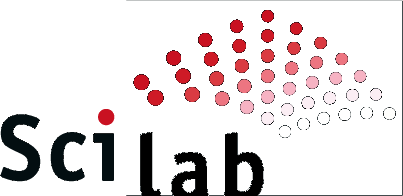
\includegraphics[height=.8cm]{png/logo_scilab}} 
\rotatebox{90}{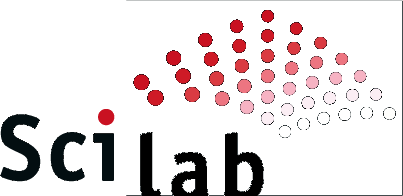
\includegraphics[height=.6cm]{png/logo_scilab}} 
        {\color{violetf}\vrule width 3pt}%
        \hspace{0pt}%must no space.
        \fboxsep=\FrameSep\colorbox{violetc}%
    }%
    \MakeFramed{\hsize #1 \advance\hsize-\width\FrameRestore}%
}%
{\endMakeFramed}%

\newenvironment{pseudo}[1][\hsize]%
{%
    \def\FrameCommand%
    {%
\rotatebox{90}{\textit{\textsf{Pseudo Code}}} 
        {\color{violetf}\vrule width 3pt}%
        \hspace{0pt}%must no space.
        \fboxsep=\FrameSep\colorbox{violetc}%
    }%
    \MakeFramed{\hsize #1 \advance\hsize-\width\FrameRestore}%
}%
{\endMakeFramed}%

\newenvironment{py}[1][\hsize]%
{%prof
    \def\FrameCommand%
    {%
%\rotatebox{90}{\textit{\textsf{Python}}} 
\rotatebox{90}{
\includegraphics[height=.6cm]{png/logo_python}} 
        {\color{violetf}\vrule width 3pt}%
        \hspace{0pt}%must no space.
        \fboxsep=\FrameSep\colorbox{violetc}%
    }%
    \MakeFramed{\hsize #1 \advance\hsize-\width\FrameRestore}%
}%
{\endMakeFramed}%


\newenvironment{term}[1][\hsize]%
{%
    \def\FrameCommand%
    {%
\rotatebox{90}{\textit{\textsf{Terminal}}} 
        {\color{violetf}\vrule width 3pt}%
        \hspace{0pt}%must no space.
        \fboxsep=\FrameSep\colorbox{violetc}%
    }%
    \MakeFramed{\hsize #1 \advance\hsize-\width\FrameRestore}%
}%
{\endMakeFramed}%


\newenvironment{rem}[1][\hsize]%
{%
    \def\FrameCommand
    {%
\rotatebox{90}{\textit{\textsf{Remarque}}} 
        {\color{bleuf}\vrule width 3pt}%
        \hspace{0pt}%must no space.
        \fboxsep=\FrameSep\colorbox{bleuc}%
    }%
    \MakeFramed{\hsize#1\advance\hsize-\width\FrameRestore}%
}%
{\endMakeFramed}%


\newenvironment{savoir}[1][\hsize]%
{%
    \def\FrameCommand
    {%
\rotatebox{90}{\textit{\textsf{Savoir}}} 
        {\color{bleuf}\vrule width 3pt}%
        \hspace{0pt}%must no space.
        \fboxsep=\FrameSep\colorbox{bleuc}%
    }%
    \MakeFramed{\hsize#1\advance\hsize-\width\FrameRestore}%
}%
{\endMakeFramed}%

\newenvironment{Objectif}[1][\hsize]%
{%
    \def\FrameCommand
    {%
\rotatebox{90}{\textit{\textsf{Objectif}}} 
        {\color{bleuf}\vrule width 3pt}%
        \hspace{0pt}%must no space.
        \fboxsep=\FrameSep\colorbox{bleuc}%
    }%
    \MakeFramed{\hsize#1\advance\hsize-\width\FrameRestore}%
}%
{\endMakeFramed}%

\newenvironment{prob}[1][\hsize]%prof
{%
    \def\FrameCommand%
    {%
\rotatebox{90}{\textit{\textsf{ Problématique}}} 
        {\color{rougef}\vrule width 3pt}%
        \hspace{0pt}%must no space.
        \fboxsep=\FrameSep\colorbox{rougec}%
    }%
    \MakeFramed{\hsize#1\advance\hsize-\width\FrameRestore}%
}%
{\endMakeFramed}%

\newenvironment{obj}[1][\hsize]%
{%
    \def\FrameCommand%
    {%
\rotatebox{90}{\textit{\textsf{ $\;$}}} 
        {\color{rougef}\vrule width 3pt}%
        \hspace{0pt}%must no space.
        \fboxsep=\FrameSep\colorbox{rougec}%
    }%
    \MakeFramed{\hsize#1\advance\hsize-\width\FrameRestore}%
}%
{\endMakeFramed}%

\newenvironment{defi}[1][\hsize]%
{%
    \def\FrameCommand%
    {%
\rotatebox{90}{\textit{\textsf{Définition\\}}} 
        {\color{bleuf}\vrule width 3pt}%
        \hspace{0pt}%must no space.
        \fboxsep=\FrameSep\colorbox{bleuc}%
    }%
    \MakeFramed{\hsize#1\advance\hsize-\width\FrameRestore}%
}%
{\endMakeFramed}%


\newenvironment{demo}[1][\hsize]%
{%
    \def\FrameCommand%
    {%
\rotatebox{90}{\textit{\textsf{Démonstration\\}}} 
        {\color{bleuf}\vrule width 3pt}%
        \hspace{0pt}%must no space.
        \fboxsep=\FrameSep\colorbox{bleuc}%
    }%
    \MakeFramed{\hsize#1\advance\hsize-\width\FrameRestore}%
}%
{\endMakeFramed}%


\newenvironment{hypo}[1][\hsize]%
{%
    \def\FrameCommand%
    {%
\rotatebox{90}{\textit{\textsf{Hypothèse\\}}} 
        {\color{bleuf}\vrule width 3pt}%
        \hspace{0pt}%must no space.
        \fboxsep=\FrameSep\colorbox{bleuc}%
    }%
    \MakeFramed{\hsize#1\advance\hsize-\width\FrameRestore}%
}%
{\endMakeFramed}%


\newenvironment{prop}[1][\hsize]%
{%
    \def\FrameCommand%
    {%
\rotatebox{90}{\textit{\textsf{Propriété\\}}} 
        {\color{bleuf}\vrule width 3pt}%
        \hspace{0pt}%must no space.
        \fboxsep=\FrameSep\colorbox{bleuc}%
    }%
    \MakeFramed{\hsize#1\advance\hsize-\width\FrameRestore}%
}%
{\endMakeFramed}%

\newenvironment{props}[1][\hsize]%
{%
    \def\FrameCommand%
    {%
\rotatebox{90}{\textit{\textsf{Propriétés\\}}} 
        {\color{bleuf}\vrule width 3pt}%
        \hspace{0pt}%must no space.
        \fboxsep=\FrameSep\colorbox{bleuc}%
    }%
    \MakeFramed{\hsize#1\advance\hsize-\width\FrameRestore}%
}%
{\endMakeFramed}%

\newenvironment{exemple}[1][\hsize]%
{%
    \def\FrameCommand%
    {%
\rotatebox{90}{\textit{\textsf{Exemple\\}}} 
        {\color{vertf}\vrule width 3pt}%
        \hspace{0pt}%must no space.
        \fboxsep=\FrameSep\colorbox{vertc}%
    }%
    \MakeFramed{\hsize#1\advance\hsize-\width\FrameRestore}%
}%
{\endMakeFramed}%

\newenvironment{exercice}[1][\hsize]%
{%
    \def\FrameCommand%
    {%
\rotatebox{90}{\textit{\textsf{Exercice\\}}} 
        {\color{vertf}\vrule width 3pt}%
        \hspace{0pt}%must no space.
        \fboxsep=\FrameSep\colorbox{vertc}%
    }%
    \MakeFramed{\hsize#1\advance\hsize-\width\FrameRestore}%
}%
{\endMakeFramed}%

\newenvironment{Support}[1][\hsize]%
{%
    \def\FrameCommand%
    {%
\rotatebox{90}{\textit{\textsf{Support de cours\\}}} 
        {\color{vertf}\vrule width 3pt}%
        \hspace{0pt}%must no space.
        \fboxsep=\FrameSep\colorbox{jaunec}%
    }%
    \MakeFramed{\hsize#1\advance\hsize-\width\FrameRestore}%
}%
{\endMakeFramed}%

\newenvironment{resultat}[1][\hsize]%
{%
    \def\FrameCommand%
    {%
\rotatebox{90}{\textit{\textsf{Résultat\\}}} 
        {\color{rougef}\vrule width 3pt}%
        \hspace{0pt}%must no space.
        \fboxsep=\FrameSep\colorbox{rougec}%
    }%
    \MakeFramed{\hsize#1\advance\hsize-\width\FrameRestore}%
}%
{\endMakeFramed}%

\newenvironment{methode}[1][\hsize]%
{%
    \def\FrameCommand%
    {%
\rotatebox{90}{\textit{\textsf{Méthode\\}}} 
        {\color{rougef}\vrule width 3pt}%
        \hspace{0pt}%must no space.
        \fboxsep=\FrameSep\colorbox{rougec}%
    }%
    \MakeFramed{\hsize#1\advance\hsize-\width\FrameRestore}%
}%
{\endMakeFramed}%

\newenvironment{theo}[1][\hsize]%
{%
    \def\FrameCommand%
    {%
\rotatebox{90}{\textit{\textsf{Théorème\\}}} 
        {\color{rougef}\vrule width 3pt}%
        \hspace{0pt}%must no space.
        \fboxsep=\FrameSep\colorbox{rougec}%
    }%
    \MakeFramed{\hsize#1\advance\hsize-\width\FrameRestore}%
}%
{\endMakeFramed}%

\newenvironment{warn}[1][\hsize]%
{%
    \def\FrameCommand%
    {%
\rotatebox{90}{\textit{\textsf{Attention\\}}} 
        {\color{rougef}\vrule width 3pt}%
        \hspace{0pt}%must no space.
        \fboxsep=\FrameSep\colorbox{rougec}%
    }%
    \MakeFramed{\hsize#1\advance\hsize-\width\FrameRestore}%
}%
{\endMakeFramed}%

% \usepackage{pstricks}
%\usepackage{minitoc}
% \setcounter{minitocdepth}{4}

\setcounter{tocdepth}{2}

% \mtcselectlanguage{french} 

%\usepackage{draftcopy}% "Brouillon"
% \usepackage{floatflt}
\usepackage{psfrag}
%\usepackage{listings} % Permet d'insérer du code de programmation
\renewcommand{\baselinestretch}{1.2}

% Changer la numérotation des figures :
% ------------------------------------
% \makeatletter
% \renewcommand{\thefigure}{\ifnum \c@section>\z@ \thesection.\fi
%  \@arabic\c@figure}
% \@addtoreset{figure}{section}
% \makeatother
 


%%%%%%%%%%%%
% Définition des vecteurs %
%%%%%%%%%%%%
 \newcommand{\vect}[1]{\overrightarrow{#1}}

%%%%%%%%%%%%
% Définition des torseusr %
%%%%%%%%%%%%

 \newcommand{\torseur}[1]{%
\left\{{#1}\right\}
}

\newcommand{\torseurcin}[3]{%
\left\{\mathcal{#1} \left(#2/#3 \right) \right\}
}

\newcommand{\torseurstat}[3]{%
\left\{\mathcal{#1} \left(#2\rightarrow #3 \right) \right\}
}

 \newcommand{\torseurc}[8]{%
%\left\{#1 \right\}=
\left\{
{#1}
\right\}
 = 
\left\{%
\begin{array}{cc}%
{#2} & {#5}\\%
{#3} & {#6}\\%
{#4} & {#7}\\%
\end{array}%
\right\}_{#8}%
}

 \newcommand{\torseurcol}[7]{
\left\{%
\begin{array}{cc}%
{#1} & {#4}\\%
{#2} & {#5}\\%
{#3} & {#6}\\%
\end{array}%
\right\}_{#7}%
}

 \newcommand{\torseurl}[3]{%
%\left\{\mathcal{#1}\right\}_{#2}=%
\left\{%
\begin{array}{l}%
{#1} \\%
{#2} %
\end{array}%
\right\}_{#3}%
}

 \newcommand{\vectv}[3]{%
\vect{V\left( {#1} \in {#2}/{#3}\right)}
}


\newcommand{\vectf}[2]{%
\vect{R\left( {#1} \rightarrow {#2}\right)}
}

\newcommand{\vectm}[3]{%
\vect{\mathcal{M}\left( {#1}, {#2} \rightarrow {#3}\right)}
}


 \newcommand{\vectg}[3]{%
\vect{\Gamma \left( {#1} \in {#2}/{#3}\right)}
}

 \newcommand{\vecto}[2]{%
\vect{\Omega\left( {#1}/{#2}\right)}
}
% }$$\left\{\mathcal{#1} \right\}_{#2} =%
% \left\{%
% \begin{array}{c}%
%  #3 \\%
%  #4 %
% \end{array}%
% \right\}_{#5}}

%  ------------------------------------------
% | Modification du formatage des sections : | 
%  ------------------------------------------

% Grands titres :
% ---------------

\newcommand{\titre}[1]{%
\begin{center}
      \bigskip
      \rule{\textwidth}{1pt}
      \par\vspace{0.1cm}
      
      \textbf{\large #1}
      \par\rule{\textwidth}{1pt}
    \end{center}
    \bigskip
  }

% Supprime le numéro du chapitre dans la numérotation des sections:
% -----------------------------------------------------------------
\makeatletter
\renewcommand{\thesection}{\@arabic\c@section}
\makeatother


% \titleformat{\chapter}[display]
% {\normalfont\Large\filcenter}
% {}
% {1pc}
% {\titlerule[1pt]
%   \vspace{1pc}%
%   \Huge}[\vspace{1ex}%
% \titlerule]


%%%% Chapitres Comme PY Pechard %%%%%%%%%
% numéro du chapitre
\DeclareFixedFont{\chapnumfont}{OT1}{phv}{b}{n}{80pt}
% pour le mot « Chapitre »
\DeclareFixedFont{\chapchapfont}{OT1}{phv}{m}{it}{40pt}
% pour le titre
\DeclareFixedFont{\chaptitfont}{T1}{phv}{b}{n}{25pt}

\definecolor{gris}{gray}{0.75}
\titleformat{\chapter}[display]%
	{\sffamily}%
	{\filleft\chapchapfont\color{gris}\chaptertitlename\
	\\
	\vspace{12pt}
	\chapnumfont\thechapter}%
	{16pt}%
	{\filleft\chaptitfont}%
	[\vspace{6pt}\titlerule\titlerule\titlerule]

%%%%  Fin Chapitres Comme PY Pechard %%%%%%%%%


% Section, subsection, subsubsection sans serifs :
% % ----------------------------------------------

% \makeatletter
% \renewcommand{\section}{\@startsection{section}{0}{0mm}%
% {\baselineskip}{.3\baselineskip}%
% {\normalfont\sffamily\Large\textbf}}%
% \makeatother

\makeatletter
\renewcommand{\@seccntformat}[1]{{\textcolor{bleu}{\csname
the#1\endcsname}\hspace{0.5em}}}
\makeatother

\makeatletter
\renewcommand{\section}{\@startsection{section}{1}{\z@}%
                       {-4ex \@plus -1ex \@minus -.4ex}%
                       {1ex \@plus.2ex }%
                       {\normalfont\Large\sffamily\bfseries}}%
\makeatother
 
\makeatletter
\renewcommand{\subsection}{\@startsection {subsection}{2}{\z@}
                          {-3ex \@plus -0.1ex \@minus -.4ex}%
                          {0.5ex \@plus.2ex }%
                          {\normalfont\large\sffamily\bfseries}}
\makeatother
 
\makeatletter
\renewcommand{\subsubsection}{\@startsection {subsubsection}{3}{\z@}
                          {-2ex \@plus -0.1ex \@minus -.2ex}%
                          {0.2ex \@plus.2ex }%
                          {\normalfont\large\sffamily\bfseries}}
\makeatother
 
\makeatletter             
\renewcommand{\paragraph}{\@startsection{paragraph}{4}{\z@}%
                                    {-2ex \@plus-.2ex \@minus .2ex}%
                                    {0.1ex}%               
{\normalfont\sffamily\bfseries}}
\makeatother
 



\makeatletter             
\renewcommand{\subparagraph}{\@startsection{subparagraph}{5}{\z@}%
                                    {-2ex \@plus-.2ex \@minus .2ex}%
                                    {0.1ex}%               
{\normalfont\bfseries Question }}
\makeatother
\renewcommand{\thesubparagraph}{\arabic{subparagraph}} 
\makeatletter

\setcounter{secnumdepth}{5}


%  --------
% | Marges |
%  --------


% \setmarginsrb{2.5cm}{1.5cm}{2.5cm}{2cm}{1cm}{1cm}{1cm}{1cm}
\setmarginsrb{1.5cm}{1cm}{1cm}{1.5cm}{1cm}{1cm}{1cm}{1cm}

% Changer les marges localement :
% -----------------------------
\newenvironment{changemargin}[2]{\begin{list}{}{%
\setlength{\topsep}{0pt}%
\setlength{\leftmargin}{0pt}%
\setlength{\rightmargin}{0pt}%
\setlength{\listparindent}{\parindent}%
\setlength{\itemindent}{\parindent}%
\setlength{\parsep}{0pt plus 1pt}%
\addtolength{\leftmargin}{#1}%
\addtolength{\rightmargin}{#2}%
}\item }{\end{list}}



\usepackage{pst-solides3d}
\usepackage{titletoc}
\titlecontents{chapter}[+3pc]
  {\addvspace{10pt}\sffamily\bfseries}
{\contentslabel[{\pscirclebox[fillstyle=solid,fillcolor=gray!25,
linecolor=gray!25,framesep=4pt]{\textcolor{white}{\thecontentslabel}}}]{2.5pc}}
  {}
  {\dotfill \normalfont\thecontentspage\ }

\titlecontents{section}[3pc]
  {\addvspace{2pt}\sffamily}
  {\contentslabel[\thecontentslabel]{1.8pc}}
  {}
  {\dotfill \normalfont\thecontentspage\ }

\titlecontents{subsection}[5pc]
  {\addvspace{2pt}\sffamily}
  {\contentslabel[\thecontentslabel]{1.8pc}}
  {}
  {\dotfill \normalfont\thecontentspage\ }

\titlecontents{subsubsection}[8pc]
  {\addvspace{2pt}\sffamily}
  {\contentslabel[\thecontentslabel]{3pc}}
  {}
  {\dotfill \normalfont\thecontentspage\ }
%{\;\titlerule\;\normalfont\thecontentspage\ }

\titlecontents{paragraph}[9pc]
  {\addvspace{2pt}\sffamily}
  {\contentslabel[\thecontentslabel]{3.5pc}}
  {}
  {\dotfill \normalfont\thecontentspage\ }

%pour avoir l indentation dans minipage
\newdimen\oldparindent\oldparindent=\parindent

\makeatletter
\def\@iiiminipage#1#2[#3]#4{%
  \noindent
  \leavevmode
  \@pboxswfalse
  \setlength\@tempdima{#4}%
  \def\@mpargs{{#1}{#2}[#3]{#4}}%
  \setbox\@tempboxa\vbox\bgroup
    \color@begingroup
      \hsize\@tempdima
      \textwidth\hsize \columnwidth\hsize
      \@parboxrestore
      \parindent=\oldparindent
      \def\@mpfn{mpfootnote}\def\thempfn{\thempfootnote}\c@mpfootnote\z@
      \let\@footnotetext\@mpfootnotetext
      \let\@listdepth\@mplistdepth \@mplistdepth\z@
      \@minipagerestore
      \@setminipage}
\makeatother

%Definition de la commande question
\newcounter{Qu}
\newcommand{\Question}[2][0]{
\ifthenelse{\equal{#1}{0}}                      %demande-t-on une minipage ?
{\medskip\noindent {\refstepcounter{Qu}\textbf{Q\theQu .\hspace{0,7mm}}#2}\ifshowanswers \else \smallskip \fi}  %non donc on balance le texte
{\ifshowanswers                                 %oui minipage en mode problem
\noindent {\refstepcounter{Qu}\textbf{Q\theQu .\hspace{0,7mm}}#2}    %mode solution
\else                                           %mode problem
\noindent\begin{minipage}{#1}\noindent {\refstepcounter{Qu}\textbf{Q\theQu .\hspace{0,7mm}}#2}\end{minipage}\smallskip
\fi }
}

\newcommand{\Questionpb}[2][0]{%le premier argument entre [] est par défaut à 0
\begin{onlyproblem}\Question[#1]{#2}\end{onlyproblem}
}

\newcommand{\Onlyproblem}[2][0]{%le premier argument entre [] est par défaut à 0
%si le 2e arguement est 0
\ifthenelse{\equal{#1}{0}}
%on demande un environnement pb classique
{\begin{onlyproblem}#2\end{onlyproblem}}
%sinon on demande à faire une minipage
{\begin{onlyproblem}\noindent\begin{minipage}{#1}\parskip2ex #2\end{minipage}\smallskip \end{onlyproblem} }
}

\newcounter{Sl}
\addtocounter{Sl}{+1}
\newcommand{\Solutioncnt}[1]{\bigskip\noindent \textbf{R\theSl .\hspace{0,7mm}}\addtocounter{Sl}{+1} #1}
\newcommand{\Solutionnorm}[1]{#1}

\newif\ifmixte
\let\mixte\mixtetrue
\let\nomix\mixtefalse
\nomix

\newcommand{\Solution}[1]{
\noindent
\ifmixte
\noindent\rule[0.1cm]{17cm}{0.8pt}\\
  \begin{solution}
    \ifnum\theQu>0
    \Solutionnorm{#1}
    \else
    \Solutioncnt{#1}
    \fi
    \smallskip
  \end{solution}

\noindent\rule[0.1cm]{17cm}{0.8pt}
\else
  \begin{onlysolution}
\fbox{\parbox{\linewidth-2\fboxrule-2\fboxsep}{
    \ifnum\theQu>0
    \Solutionnorm{#1}
    \else
    \Solutioncnt{#1}
    \fi
    \smallskip
}}
  \end{onlysolution}
\fi
}

%\usepackage{algorithm}
%\usepackage{algorithmic}
\usepackage[french]{algorithm2e}

\SetKwBlock{Fonction}{Début Fonction}{Fin Fonction}
\SetKwComment{Comment}{start}{end}
% Python sources

\usepackage{listings}
\lstloadlanguages{R}   % pour regler les pb d accent utf8 dans les codes
\lstset{language=R} % pour regler les pb d accent utf8 dans les codes

\usepackage{textcomp}
\usepackage{setspace}
%\usepackage{palatino}

%\usepackage{color}
\definecolor{Bleu}{rgb}{0.1,0.1,1.0}
\definecolor{Noir}{rgb}{0,0,0}
\definecolor{Grau}{rgb}{0.5,0.5,0.5}
\definecolor{DunkelGrau}{rgb}{0.15,0.15,0.15}
\definecolor{Hellbraun}{rgb}{0.5,0.25,0.0}
\definecolor{Magenta}{rgb}{1.0,0.0,1.0}
\definecolor{Gris}{gray}{0.5}
\definecolor{Vert}{rgb}{0,0.5,0}
\definecolor{SourceHintergrund}{rgb}{1,1.0,0.95}


%
\renewcommand{\lstlistlistingname}{Listings}
\renewcommand{\lstlistingname}{Listing}

\lstnewenvironment{python}[1][]{
\lstset{
%escapeinside={\%*}{*)},
%inputencoding=utf8,   % pour regler les pb d accent utf8 dans les codes
%extendedchars=true,   % pour regler les pb d accent utf8 dans les codes
language=python,
basicstyle=\sffamily\footnotesize, 	
stringstyle=\color{red}, 
showstringspaces=false, 
alsoletter={1234567890},
otherkeywords={\ , \}, \{},
keywordstyle=\color{blue},
emph={access,and,break,class,continue,def,del,elif ,else,
except,exec,finally,for,from,global,if,import,in,i s,
lambda,not,or,pass,print,raise,return,try,while},
emphstyle=\color{black}\bfseries,
emph={[2]True, False, None, self},
emphstyle=[2]\color{olive},
emph={[3]from, import, as},
emphstyle=[3]\color{blue},
upquote=true,
columns=flexible, % pour empecher d'avoir un espacement mono
morecomment=[s]{"""}{"""},
commentstyle=\color{Hellbraun}\slshape, 
%emph={[4]1, 2, 3, 4, 5, 6, 7, 8, 9, 0},
emphstyle=[4]\color{blue},
literate=*{:}{{\textcolor{blue}:}}{1}
{=}{{\textcolor{blue}=}}{1}
{-}{{\textcolor{blue}-}}{1}
{+}{{\textcolor{blue}+}}{1}
{*}{{\textcolor{blue}*}}{1}
{!}{{\textcolor{blue}!}}{1}
{(}{{\textcolor{blue}(}}{1}
{)}{{\textcolor{blue})}}{1}
{[}{{\textcolor{blue}[}}{1}
{]}{{\textcolor{blue}]}}{1}
{<}{{\textcolor{blue}<}}{1}
{>}{{\textcolor{blue}>}}{1}
{COMPLETER}{{\textcolor{red}COMPLETER}}{1},
literate=%
            {é}{{\'{e}}}1
            {è}{{\`{e}}}1
            {ê}{{\^{e}}}1
            {ë}{{\¨{e}}}1
            {û}{{\^{u}}}1
            {ù}{{\`{u}}}1
            {â}{{\^{a}}}1
            {à}{{\`{a}}}1
            {î}{{\^{i}}}1
            {ç}{{\c{c}}}1
            {Ç}{{\c{C}}}1
            {É}{{\'{E}}}1
            {Ê}{{\^{E}}}1
            {À}{{\`{A}}}1
            {Â}{{\^{A}}}1
            {Î}{{\^{I}}}1, % pour regler les pb d accent utf8 dans les codes
%framexleftmargin=1mm, framextopmargin=1mm, frame=shadowbox, rulesepcolor=\color{blue},#1
%backgroundcolor=\color{SourceHintergrund}, 
%framexleftmargin=1mm, framexrightmargin=1mm, framextopmargin=1mm, frame=single, framerule=1pt, rulecolor=\color{black},#1
}}{}



\lstnewenvironment{scilab}[1][]{
\lstset{
language=scilab,
basicstyle=\sffamily\footnotesize, 	
stringstyle=\color{red}, 
showstringspaces=false, 
alsoletter={1234567890},
otherkeywords={\ , \}, \{},
keywordstyle=\color{blue},
emph={access,and,break,class,continue,def,del,elif ,else,
except,exec,finally,for,from,global,if,import,in,i s,
lambda,not,or,pass,print,raise,return,try,while,Debut},
emphstyle=\color{black}\bfseries,
emph={[2]True, False, None, self},
emphstyle=[2]\color{olive},
emph={[3]from, import, as},
emphstyle=[3]\color{blue},
upquote=true,
columns=flexible, % pour empecher d'avoir un espacement mono
morecomment=[s]{"""}{"""},
commentstyle=\color{Hellbraun}\slshape, 
%emph={[4]1, 2, 3, 4, 5, 6, 7, 8, 9, 0},
emphstyle=[4]\color{blue},
literate=*{:}{{\textcolor{blue}:}}{1}
{=}{{\textcolor{blue}=}}{1}
{-}{{\textcolor{blue}-}}{1}
{+}{{\textcolor{blue}+}}{1}
{*}{{\textcolor{blue}*}}{1}
{!}{{\textcolor{blue}!}}{1}
{(}{{\textcolor{blue}(}}{1}
{)}{{\textcolor{blue})}}{1}
{[}{{\textcolor{blue}[}}{1}
{]}{{\textcolor{blue}]}}{1}
{<}{{\textcolor{blue}<}}{1}
{>}{{\textcolor{blue}>}}{1},
%framexleftmargin=1mm, framextopmargin=1mm, frame=shadowbox, rulesepcolor=\color{blue},#1
%backgroundcolor=\color{SourceHintergrund}, 
%framexleftmargin=1mm, framexrightmargin=1mm, framextopmargin=1mm, frame=single, framerule=1pt, rulecolor=\color{black},#1
}}{}


\lstdefinestyle{stylepython}{%
escapeinside={\%*}{*)},
inputencoding=utf8,   % pour regler les pb d accent utf8 dans les codes
extendedchars=true,   % pour regler les pb d accent utf8 dans les codes
language=python,
basicstyle=\sffamily\footnotesize, 	
stringstyle=\color{red}, 
showstringspaces=false, 
alsoletter={1234567890},
otherkeywords={\ , \}, \{},
keywordstyle=\color{blue},
emph={access,and,break,class,continue,def,del,elif ,else,
except,exec,finally,for,from,global,if,import,in,i s,
lambda,not,or,pass,print,raise,return,try,while},
emphstyle=\color{black}\bfseries,
emph={[2]True, False, None, self},
emphstyle=[2]\color{green},
emph={[3]from, import, as},
emphstyle=[3]\color{blue},
upquote=true,
columns=flexible, % pour empecher d'avoir un espacement mono
morecomment=[s]{"""}{"""},
commentstyle=\color{Hellbraun}\slshape, 
%emph={[4]1, 2, 3, 4, 5, 6, 7, 8, 9, 0},
emphstyle=[4]\color{blue},
literate=*{:}{{\textcolor{blue}:}}{1}
{=}{{\textcolor{blue}=}}{1}
{-}{{\textcolor{blue}-}}{1}
{+}{{\textcolor{blue}+}}{1}
{*}{{\textcolor{blue}*}}{1}
{!}{{\textcolor{blue}!}}{1}
{(}{{\textcolor{blue}(}}{1}
{)}{{\textcolor{blue})}}{1}
{[}{{\textcolor{blue}[}}{1}
{]}{{\textcolor{blue}]}}{1}
{<}{{\textcolor{blue}<}}{1}
{>}{{\textcolor{blue}>}}{1}
{COMPLETER}{{\textcolor{red}COMPLETER}}{1},
literate=%
            {é}{{\'{e}}}1
            {è}{{\`{e}}}1
            {ê}{{\^{e}}}1
            {ë}{{\¨{e}}}1
            {û}{{\^{u}}}1
            {ù}{{\`{u}}}1
            {â}{{\^{a}}}1
            {à}{{\`{a}}}1
            {î}{{\^{i}}}1
            {ç}{{\c{c}}}1
            {Ç}{{\c{C}}}1
            {É}{{\'{E}}}1
            {Ê}{{\^{E}}}1
            {À}{{\`{A}}}1
            {Â}{{\^{A}}}1
            {Î}{{\^{I}}}1,
%numbers=left,                    % where to put the line-numbers; possible values are (none, left, right)
%numbersep=5pt,                   % how far the line-numbers are from the code
%numberstyle=\tiny\color{mygray}, % the style that is used for the line-numbers
}

%
%\renewcommand{\algorithmicrequire} {\textbf{\textsc{Entrées:}}}
%\renewcommand{\algorithmicensure}  {\textbf{\textsc{Sorties:}}}
%\renewcommand{\algorithmicwhile}   {\textbf{tantque}}
%\renewcommand{\algorithmicdo}      {\textbf{faire}}
%\renewcommand{\algorithmicendwhile}{\textbf{fin tantque}}
%\renewcommand{\algorithmicend}     {\textbf{fin}}
%\renewcommand{\algorithmicif}      {\textbf{si}}
%\renewcommand{\algorithmicendif}   {\textbf{finsi}}
%\renewcommand{\algorithmicelse}    {\textbf{sinon}}
%\renewcommand{\algorithmicthen}    {\textbf{alors}}
%\renewcommand{\algorithmicfor}     {\textbf{pour}}
%\renewcommand{\algorithmicforall}  {\textbf{pour tout}}
%\renewcommand{\algorithmicdo}      {\textbf{faire}}
%\renewcommand{\algorithmicendfor}  {\textbf{fin pour}}
%\renewcommand{\algorithmicloop}    {\textbf{boucler}}
%\renewcommand{\algorithmicendloop} {\textbf{fin boucle}}
%\renewcommand{\algorithmicrepeat}  {\textbf{répéter}}
%\renewcommand{\algorithmicuntil}   {\textbf{jusqu'à}}

\lstnewenvironment{termi}[1][]{
\lstset{
language=scilab,
basicstyle=\sffamily\footnotesize, 	
stringstyle=\color{red}, 
showstringspaces=false, 
alsoletter={1234567890},
otherkeywords={\ , \}, \{},
keywordstyle=\color{blue},
emph={access,and,break,class,continue,def,del,elif ,else,
except,exec,finally,for,from,global,if,import,in,i s,
lambda,not,or,pass,print,raise,return,try,while,Debut},
emphstyle=\color{black}\bfseries,
emph={[2]True, False, None, self},
emphstyle=[2]\color{green},
emph={[3]from, import, as},
emphstyle=[3]\color{blue},
upquote=true,
columns=flexible, % pour empecher d'avoir un espacement mono
morecomment=[s]{"""}{"""},
commentstyle=\color{Hellbraun}\slshape, 
%emph={[4]1, 2, 3, 4, 5, 6, 7, 8, 9, 0},
emphstyle=[4]\color{blue},
literate=*{:}{{\textcolor{blue}:}}{1}
{=}{{\textcolor{blue}=}}{1}
{-}{{\textcolor{blue}-}}{1}
{+}{{\textcolor{blue}+}}{1}
{*}{{\textcolor{blue}*}}{1}
{!}{{\textcolor{blue}!}}{1}
{(}{{\textcolor{blue}(}}{1}
{)}{{\textcolor{blue})}}{1}
{[}{{\textcolor{blue}[}}{1}
{]}{{\textcolor{blue}]}}{1}
{<}{{\textcolor{blue}<}}{1}
{>}{{\textcolor{blue}>}}{1},
%framexleftmargin=1mm, framextopmargin=1mm, frame=shadowbox, rulesepcolor=\color{blue},#1
%backgroundcolor=\color{SourceHintergrund}, 
%framexleftmargin=1mm, framexrightmargin=1mm, framextopmargin=1mm, frame=single, framerule=1pt, rulecolor=\color{black},#1
}}{}


\lstnewenvironment{sql}[1][]{
\lstset{
%escapeinside={\%*}{*)},
%inputencoding=utf8,   % pour regler les pb d accent utf8 dans les codes
%extendedchars=true,   % pour regler les pb d accent utf8 dans les codes
language=sql,
basicstyle=\sffamily\footnotesize, 	
stringstyle=\color{red}, 
showstringspaces=false, 
alsoletter={1234567890},
otherkeywords={\ , \}, \{},
keywordstyle=\color{blue},
emph={access,and,break,class,continue,def,del,elif ,else,
except,exec,finally,for,from,global,if,import,in,i s,
lambda,not,or,pass,print,raise,return,try,while},
emphstyle=\color{black}\bfseries,
emph={[2]True, False, None, self},
emphstyle=[2]\color{olive},
emph={[3]from, import, as},
emphstyle=[3]\color{blue},
upquote=true,
columns=flexible, % pour empecher d'avoir un espacement mono
morecomment=[s]{"""}{"""},
commentstyle=\color{Hellbraun}\slshape, 
%emph={[4]1, 2, 3, 4, 5, 6, 7, 8, 9, 0},
emphstyle=[4]\color{blue},
literate=*{:}{{\textcolor{blue}:}}{1}
{=}{{\textcolor{blue}=}}{1}
{-}{{\textcolor{blue}-}}{1}
{+}{{\textcolor{blue}+}}{1}
{*}{{\textcolor{blue}*}}{1}
{!}{{\textcolor{blue}!}}{1}
{(}{{\textcolor{blue}(}}{1}
{)}{{\textcolor{blue})}}{1}
{[}{{\textcolor{blue}[}}{1}
{]}{{\textcolor{blue}]}}{1}
{<}{{\textcolor{blue}<}}{1}
{>}{{\textcolor{blue}>}}{1}
{COMPLETER}{{\textcolor{red}COMPLETER}}{1},
literate=%
            {é}{{\'{e}}}1
            {è}{{\`{e}}}1
            {ê}{{\^{e}}}1
            {ë}{{\¨{e}}}1
            {û}{{\^{u}}}1
            {ù}{{\`{u}}}1
            {â}{{\^{a}}}1
            {à}{{\`{a}}}1
            {î}{{\^{i}}}1
            {ç}{{\c{c}}}1
            {Ç}{{\c{C}}}1
            {É}{{\'{E}}}1
            {Ê}{{\^{E}}}1
            {À}{{\`{A}}}1
            {Â}{{\^{A}}}1
            {Î}{{\^{I}}}1, % pour regler les pb d accent utf8 dans les codes
%framexleftmargin=1mm, framextopmargin=1mm, frame=shadowbox, rulesepcolor=\color{blue},#1
%backgroundcolor=\color{SourceHintergrund}, 
%framexleftmargin=1mm, framexrightmargin=1mm, framextopmargin=1mm, frame=single, framerule=1pt, rulecolor=\color{black},#1
}}{}


%
%\renewcommand{\algorithmicrequire} {\textbf{\textsc{Entrées:}}}
%\renewcommand{\algorithmicensure}  {\textbf{\textsc{Sorties:}}}
%\renewcommand{\algorithmicwhile}   {\textbf{tantque}}
%\renewcommand{\algorithmicdo}      {\textbf{faire}}
%\renewcommand{\algorithmicendwhile}{\textbf{fin tantque}}
%\renewcommand{\algorithmicend}     {\textbf{fin}}
%\renewcommand{\algorithmicif}      {\textbf{si}}
%\renewcommand{\algorithmicendif}   {\textbf{finsi}}
%\renewcommand{\algorithmicelse}    {\textbf{sinon}}
%\renewcommand{\algorithmicthen}    {\textbf{alors}}
%\renewcommand{\algorithmicfor}     {\textbf{pour}}
%\renewcommand{\algorithmicforall}  {\textbf{pour tout}}
%\renewcommand{\algorithmicdo}      {\textbf{faire}}
%\renewcommand{\algorithmicendfor}  {\textbf{fin pour}}
%\renewcommand{\algorithmicloop}    {\textbf{boucler}}
%\renewcommand{\algorithmicendloop} {\textbf{fin boucle}}
%\renewcommand{\algorithmicrepeat}  {\textbf{répéter}}
%\renewcommand{\algorithmicuntil}   {\textbf{jusqu'à}}
%%%%%%%%%%%%
% Définition des vecteurs 
%%%%%%%%%%%%
 \newcommand{\vect}[1]{\overrightarrow{#1}}
\newcommand{\axe}[2]{\left(#1,\vect{#2}\right)}

\newcommand{\rep}[1]{\mathcal{R}_{#1}}
\newcommand{\vx}[1]{\vect{x_{#1}}}
\newcommand{\vy}[1]{\vect{y_{#1}}}
\newcommand{\vz}[1]{\vect{z_{#1}}}

%%%%%%%%%%%%
% Définition des torseurs 
%%%%%%%%%%%%

 \newcommand{\torseur}[1]{%
\left\{{#1}\right\}
}

\newcommand{\torseurcin}[3]{%
\left\{\mathcal{#1} \left(#2/#3 \right) \right\}
}

\newcommand{\torseurstat}[3]{%
\left\{\mathcal{#1} \left(#2\rightarrow #3 \right) \right\}
}

 \newcommand{\torseurc}[8]{%
%\left\{#1 \right\}=
\left\{
{#1}
\right\}
 = 
\left\{%
\begin{array}{cc}%
{#2} & {#5}\\%
{#3} & {#6}\\%
{#4} & {#7}\\%
\end{array}%
\right\}_{#8}%
}

 \newcommand{\torseurcol}[7]{
\left\{%
\begin{array}{cc}%
{#1} & {#4}\\%
{#2} & {#5}\\%
{#3} & {#6}\\%
\end{array}%
\right\}_{#7}%
}

 \newcommand{\torseurl}[3]{%
%\left\{\mathcal{#1}\right\}_{#2}=%
\left\{%
\begin{array}{l}%
{#1} \\%
{#2} %
\end{array}%
\right\}_{#3}%
}

 \newcommand{\vectv}[3]{%
\vect{V\left( {#1} \in {#2}/{#3}\right)}
}


\newcommand{\vectf}[2]{%
\vect{R\left( {#1} \rightarrow {#2}\right)}
}

\newcommand{\vectm}[3]{%
\vect{\mathcal{M}\left( {#1}, {#2} \rightarrow {#3}\right)}
}


 \newcommand{\vectg}[3]{%
\vect{\Gamma \left( {#1} \in {#2}/{#3}\right)}
}

 \newcommand{\vecto}[2]{%
\vect{\Omega\left( {#1}/{#2}\right)}
}
% }$$\left\{\mathcal{#1} \right\}_{#2} =%
% \left\{%
% \begin{array}{c}%
%  #3 \\%
%  #4 %
% \end{array}%
% \right\}_{#5}}
\setcounter{tocdepth}{2}
% \mtcselectlanguage{french} 


%  ------------------------------------------
% | Modification du formatage des sections : | 
%  ------------------------------------------

% Grands titres :
% ---------------

\newcommand{\titre}[1]{%
\begin{center}
      \bigskip
      \rule{\textwidth}{1pt}
      \par\vspace{0.1cm}
      
      \textbf{\large #1}
      \par\rule{\textwidth}{1pt}
    \end{center}
    \bigskip
  }

% Supprime le numéro du chapitre dans la numérotation des sections:
% -----------------------------------------------------------------
\makeatletter
\renewcommand{\thesection}{\@arabic\c@section}
\makeatother


% \titleformat{\chapter}[display]
% {\normalfont\Large\filcenter}
% {}
% {1pc}
% {\titlerule[1pt]
%   \vspace{1pc}%
%   \Huge}[\vspace{1ex}%
% \titlerule]


%%%% Chapitres Comme PY Pechard %%%%%%%%%
% numéro du chapitre
\DeclareFixedFont{\chapnumfont}{OT1}{phv}{b}{n}{80pt}
% pour le mot « Chapitre »
\DeclareFixedFont{\chapchapfont}{OT1}{phv}{m}{it}{40pt}
% pour le titre
\DeclareFixedFont{\chaptitfont}{T1}{phv}{b}{n}{25pt}

\definecolor{gris}{gray}{0.75}
\titleformat{\chapter}[display]%
	{\sffamily}%
	{\filleft\chapchapfont\color{gris}\chaptertitlename\
	\\
	\vspace{12pt}
	\chapnumfont\thechapter}%
	{16pt}%
	{\filleft\chaptitfont}%
	[\vspace{6pt}\titlerule\titlerule\titlerule]

%%%%  Fin Chapitres Comme PY Pechard %%%%%%%%%


% Section, subsection, subsubsection sans serifs :
% % ----------------------------------------------

% \makeatletter
% \renewcommand{\section}{\@startsection{section}{0}{0mm}%
% {\baselineskip}{.3\baselineskip}%
% {\normalfont\sffamily\Large\textbf}}%
% \makeatother

\makeatletter
\renewcommand{\@seccntformat}[1]{{\textcolor{bleu}{\csname
the#1\endcsname}\hspace{0.5em}}}
\makeatother

\makeatletter
\renewcommand{\section}{\@startsection{section}{1}{\z@}%
                       {-4ex \@plus -1ex \@minus -.4ex}%
                       {1ex \@plus.2ex }%
                       {\normalfont\Large\sffamily\bfseries}}%
\makeatother
 
\makeatletter
\renewcommand{\subsection}{\@startsection {subsection}{2}{\z@}
                          {-3ex \@plus -0.1ex \@minus -.4ex}%
                          {0.5ex \@plus.2ex }%
                          {\normalfont\large\sffamily\bfseries}}
\makeatother
 
\makeatletter
\renewcommand{\subsubsection}{\@startsection {subsubsection}{3}{\z@}
                          {-2ex \@plus -0.1ex \@minus -.2ex}%
                          {0.2ex \@plus.2ex }%
                          {\normalfont\large\sffamily\bfseries}}
\makeatother
 
\makeatletter             
\renewcommand{\paragraph}{\@startsection{paragraph}{4}{\z@}%
                                    {-2ex \@plus-.2ex \@minus .2ex}%
                                    {0.1ex}%               
{\normalfont\sffamily\bfseries}}
\makeatother
 
 
\makeatletter             
\renewcommand{\subparagraph}{\@startsection{subparagraph}{5}{\z@}%
                                    {-2ex \@plus-.2ex \@minus .2ex}%
                                    {0ex}%               
{\normalfont\bfseries Question }}
\makeatother
\renewcommand{\thesubparagraph}{\arabic{subparagraph}} 
\makeatletter

\setcounter{secnumdepth}{5}





% Formatage de la table des matières 
% Paquets nécessaires : titletoc ?

% Chapitre spéciaux écrits dans un nombre cerclé dans la table des matières.
\titlecontents{chapter}[+3pc]
  {\addvspace{10pt}\sffamily\bfseries}
{\contentslabel[{\pscirclebox[fillstyle=solid,fillcolor=gray!25,
linecolor=gray!25,framesep=4pt]{\textcolor{white}{\thecontentslabel}}}]{2.5pc}}
  {}
  {\dotfill \normalfont\thecontentspage\ }

\titlecontents{section}[3pc]
  {\addvspace{2pt}\sffamily}
  {\contentslabel[\thecontentslabel]{1.8pc}}
  {}
  {\dotfill \normalfont\thecontentspage\ }

\titlecontents{subsection}[5pc]
  {\addvspace{2pt}\sffamily}
  {\contentslabel[\thecontentslabel]{1.8pc}}
  {}
  {\dotfill \normalfont\thecontentspage\ }

\titlecontents{subsubsection}[8pc]
  {\addvspace{2pt}\sffamily}
  {\contentslabel[\thecontentslabel]{3pc}}
  {}
  {\dotfill \normalfont\thecontentspage\ }
%{\;\titlerule\;\normalfont\thecontentspage\ }

\titlecontents{paragraph}[9pc]
  {\addvspace{2pt}\sffamily}
  {\contentslabel[\thecontentslabel]{3.5pc}}
  {}
  {\dotfill \normalfont\thecontentspage\ }

%pour avoir l indentation dans minipage
\newdimen\oldparindent\oldparindent=\parindent

\makeatletter
\def\@iiiminipage#1#2[#3]#4{%
  \noindent
  \leavevmode
  \@pboxswfalse
  \setlength\@tempdima{#4}%
  \def\@mpargs{{#1}{#2}[#3]{#4}}%
  \setbox\@tempboxa\vbox\bgroup
    \color@begingroup
      \hsize\@tempdima
      \textwidth\hsize \columnwidth\hsize
      \@parboxrestore
      \parindent=\oldparindent
      \def\@mpfn{mpfootnote}\def\thempfn{\thempfootnote}\c@mpfootnote\z@
      \let\@footnotetext\@mpfootnotetext
      \let\@listdepth\@mplistdepth \@mplistdepth\z@
      \@minipagerestore
      \@setminipage}
\makeatother

% Paquets requis : 

\definecolor{gris25}{gray}{0.75}
\definecolor{bleu}{RGB}{18,33,98}
\definecolor{bleuf}{RGB}{42,94,171}
\definecolor{bleuc}{RGB}{231,239,247}
\definecolor{rougef}{RGB}{185,18,27}
\definecolor{rougec}{RGB}{255,230,231}
\definecolor{vertf}{RGB}{103,126,82}
\definecolor{vertc}{RGB}{220,255,191}
\definecolor{violetf}{RGB}{112,48,160}
\definecolor{violetc}{RGB}{230,224,236}
\definecolor{jaunec}{RGB}{220,255,191}

\newenvironment{sci}[1][\hsize]%
{%
    \def\FrameCommand%
    {%
%\rotatebox{90}{\textit{\textsf{Scilab}}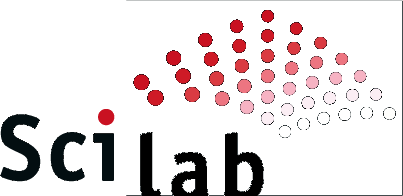
\includegraphics[height=.8cm]{png/logo_scilab}} 
\rotatebox{90}{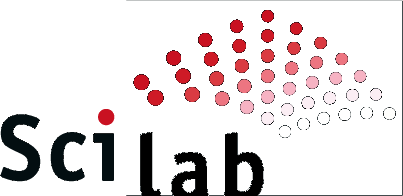
\includegraphics[height=.6cm]{png/logo_scilab}} 
        {\color{violetf}\vrule width 3pt}%
        \hspace{0pt}%must no space.
        \fboxsep=\FrameSep\colorbox{violetc}%
    }%
    \MakeFramed{\hsize #1 \advance\hsize-\width\FrameRestore}%
}%
{\endMakeFramed}%

\newenvironment{pseudo}[1][\hsize]%
{%
    \def\FrameCommand%
    {%
\rotatebox{90}{\textit{\textsf{Pseudo Code}}} 
        {\color{violetf}\vrule width 3pt}%
        \hspace{0pt}%must no space.
        \fboxsep=\FrameSep\colorbox{violetc}%
    }%
    \MakeFramed{\hsize #1 \advance\hsize-\width\FrameRestore}%
}%
{\endMakeFramed}%

\newenvironment{py}[1][\hsize]%
{%
    \def\FrameCommand%
    {%
%\rotatebox{90}{\textit{\textsf{Python}}} 
\rotatebox{90}{
\includegraphics[height=.6cm]{png/logo_python}} 
        {\color{violetf}\vrule width 3pt}%
        \hspace{0pt}%must no space.
        \fboxsep=\FrameSep\colorbox{violetc}%
    }%
    \MakeFramed{\hsize #1 \advance\hsize-\width\FrameRestore}%
}%
{\endMakeFramed}%


\newenvironment{envsql}[1][\hsize]%
{%
    \def\FrameCommand%
    {%
\rotatebox{90}{\textit{\textsf{SQL}}} 
        {\color{violetf}\vrule width 3pt}%
        \hspace{0pt}%must no space.
        \fboxsep=\FrameSep\colorbox{violetc}%
    }%
    \MakeFramed{\hsize #1 \advance\hsize-\width\FrameRestore}%
}%
{\endMakeFramed}%


\newenvironment{term}[1][\hsize]%
{%
    \def\FrameCommand%
    {%
\rotatebox{90}{\textit{\textsf{Terminal}}} 
        {\color{violetf}\vrule width 3pt}%
        \hspace{0pt}%must no space.
        \fboxsep=\FrameSep\colorbox{violetc}%
    }%
    \MakeFramed{\hsize #1 \advance\hsize-\width\FrameRestore}%
}%
{\endMakeFramed}%


\newenvironment{rem}[1][\hsize]%
{%
    \def\FrameCommand
    {%
\rotatebox{90}{\textit{\textsf{Remarque}}} 
        {\color{bleuf}\vrule width 3pt}%
        \hspace{0pt}%must no space.
        \fboxsep=\FrameSep\colorbox{bleuc}%
    }%
    \MakeFramed{\hsize#1\advance\hsize-\width\FrameRestore}%
}%
{\endMakeFramed}%


\newenvironment{savoir}[1][\hsize]%
{%
    \def\FrameCommand
    {%
\rotatebox{90}{\textit{\textsf{Savoir}}} 
        {\color{bleuf}\vrule width 3pt}%
        \hspace{0pt}%must no space.
        \fboxsep=\FrameSep\colorbox{bleuc}%
    }%
    \MakeFramed{\hsize#1\advance\hsize-\width\FrameRestore}%
}%
{\endMakeFramed}%

\newenvironment{Objectif}[1][\hsize]%
{%
    \def\FrameCommand
    {%
\rotatebox{90}{\textit{\textsf{Objectif}}} 
        {\color{bleuf}\vrule width 3pt}%
        \hspace{0pt}%must no space.
        \fboxsep=\FrameSep\colorbox{bleuc}%
    }%
    \MakeFramed{\hsize#1\advance\hsize-\width\FrameRestore}%
}%
{\endMakeFramed}%

\newenvironment{prob}[1][\hsize]%
{%
    \def\FrameCommand%
    {%
\rotatebox{90}{\textit{\textsf{ Problématique}}} 
        {\color{rougef}\vrule width 3pt}%
        \hspace{0pt}%must no space.
        \fboxsep=\FrameSep\colorbox{rougec}%
    }%
    \MakeFramed{\hsize#1\advance\hsize-\width\FrameRestore}%
}%
{\endMakeFramed}%

\newenvironment{obj}[1][\hsize]%
{%
    \def\FrameCommand%
    {%
\rotatebox{90}{\textit{\textsf{ $\;$}}} 
        {\color{rougef}\vrule width 3pt}%
        \hspace{0pt}%must no space.
        \fboxsep=\FrameSep\colorbox{rougec}%
    }%
    \MakeFramed{\hsize#1\advance\hsize-\width\FrameRestore}%
}%
{\endMakeFramed}%

\newenvironment{defi}[1][\hsize]%
{%
    \def\FrameCommand%
    {%
\rotatebox{90}{\textit{\textsf{Définition\\}}} 
        {\color{bleuf}\vrule width 3pt}%
        \hspace{0pt}%must no space.
        \fboxsep=\FrameSep\colorbox{bleuc}%
    }%
    \MakeFramed{\hsize#1\advance\hsize-\width\FrameRestore}%
}%
{\endMakeFramed}%


\newenvironment{demo}[1][\hsize]%
{%
    \def\FrameCommand%
    {%
\rotatebox{90}{\textit{\textsf{Démonstration\\}}} 
        {\color{bleuf}\vrule width 3pt}%
        \hspace{0pt}%must no space.
        \fboxsep=\FrameSep\colorbox{bleuc}%
    }%
    \MakeFramed{\hsize#1\advance\hsize-\width\FrameRestore}%
}%
{\endMakeFramed}%


\newenvironment{hypo}[1][\hsize]%
{%
    \def\FrameCommand%
    {%
\rotatebox{90}{\textit{\textsf{Hypothèse\\}}} 
        {\color{bleuf}\vrule width 3pt}%
        \hspace{0pt}%must no space.
        \fboxsep=\FrameSep\colorbox{bleuc}%
    }%
    \MakeFramed{\hsize#1\advance\hsize-\width\FrameRestore}%
}%
{\endMakeFramed}%


\newenvironment{prop}[1][\hsize]%
{%
    \def\FrameCommand%
    {%
\rotatebox{90}{\textit{\textsf{Propriété\\}}} 
        {\color{bleuf}\vrule width 3pt}%
        \hspace{0pt}%must no space.
        \fboxsep=\FrameSep\colorbox{bleuc}%
    }%
    \MakeFramed{\hsize#1\advance\hsize-\width\FrameRestore}%
}%
{\endMakeFramed}%

\newenvironment{props}[1][\hsize]%
{%
    \def\FrameCommand%
    {%
\rotatebox{90}{\textit{\textsf{Propriétés\\}}} 
        {\color{bleuf}\vrule width 3pt}%
        \hspace{0pt}%must no space.
        \fboxsep=\FrameSep\colorbox{bleuc}%
    }%
    \MakeFramed{\hsize#1\advance\hsize-\width\FrameRestore}%
}%
{\endMakeFramed}%

\newenvironment{exemple}[1][\hsize]%
{%
    \def\FrameCommand%
    {%
\rotatebox{90}{\textit{\textsf{Exemple\\}}} 
        {\color{vertf}\vrule width 3pt}%
        \hspace{0pt}%must no space.
        \fboxsep=\FrameSep\colorbox{vertc}%
    }%
    \MakeFramed{\hsize#1\advance\hsize-\width\FrameRestore}%
}%
{\endMakeFramed}%

\newenvironment{exercice}[1][\hsize]%
{%
    \def\FrameCommand%
    {%
\rotatebox{90}{\textit{\textsf{Exercice\\}}} 
        {\color{vertf}\vrule width 3pt}%
        \hspace{0pt}%must no space.
        \fboxsep=\FrameSep\colorbox{vertc}%
    }%
    \MakeFramed{\hsize#1\advance\hsize-\width\FrameRestore}%
}%
{\endMakeFramed}%

\newenvironment{Support}[1][\hsize]%
{%
    \def\FrameCommand%
    {%
\rotatebox{90}{\textit{\textsf{Support de cours\\}}} 
        {\color{vertf}\vrule width 3pt}%
        \hspace{0pt}%must no space.
        \fboxsep=\FrameSep\colorbox{jaunec}%
    }%
    \MakeFramed{\hsize#1\advance\hsize-\width\FrameRestore}%
}%
{\endMakeFramed}%

\newenvironment{resultat}[1][\hsize]%
{%
    \def\FrameCommand%
    {%
\rotatebox{90}{\textit{\textsf{Résultat\\}}} 
        {\color{rougef}\vrule width 3pt}%
        \hspace{0pt}%must no space.
        \fboxsep=\FrameSep\colorbox{rougec}%
    }%
    \MakeFramed{\hsize#1\advance\hsize-\width\FrameRestore}%
}%
{\endMakeFramed}%

\newenvironment{methode}[1][\hsize]%
{%
    \def\FrameCommand%
    {%
\rotatebox{90}{\textit{\textsf{Méthode\\}}} 
        {\color{rougef}\vrule width 3pt}%
        \hspace{0pt}%must no space.
        \fboxsep=\FrameSep\colorbox{rougec}%
    }%
    \MakeFramed{\hsize#1\advance\hsize-\width\FrameRestore}%
}%
{\endMakeFramed}%

\newenvironment{theo}[1][\hsize]%
{%
    \def\FrameCommand%
    {%
\rotatebox{90}{\textit{\textsf{Théorème\\}}} 
        {\color{rougef}\vrule width 3pt}%
        \hspace{0pt}%must no space.
        \fboxsep=\FrameSep\colorbox{rougec}%
    }%
    \MakeFramed{\hsize#1\advance\hsize-\width\FrameRestore}%
}%
{\endMakeFramed}%

\newenvironment{warn}[1][\hsize]%
{%
    \def\FrameCommand%
    {%
\rotatebox{90}{\textit{\textsf{Attention\\}}} 
        {\color{rougef}\vrule width 3pt}%
        \hspace{0pt}%must no space.
        \fboxsep=\FrameSep\colorbox{rougec}%
    }%
    \MakeFramed{\hsize#1\advance\hsize-\width\FrameRestore}%
}%
{\endMakeFramed}%


%Si le boolen xp est vrai : compilation pour xabi
%Sinon compilation Damien
\newboolean{xp}
\setboolean{xp}{true}

\newboolean{prof}
\setboolean{prof}{true}

\usepackage[%
    pdftitle={Problèmes stationnaires},
    pdfauthor={Xavier Pessoles},
    colorlinks=true,
    linkcolor=blue,
    citecolor=magenta]{hyperref}


\def\discipline{Informatique}
\def\xxtitre{\ifthenelse{\boolean{xp}}{
CI 3 : Ingénierie Numérique \& Simulation}{
Chapitre  -- }}

\def\xxsoustitre{\ifthenelse{\boolean{xp}}{
Chapitre 3 -- Résolution des équation différentielles}{
Partie  -- }}

\def\xxauteur{\ifthenelse{\boolean{xp}}{
Xavier \textsc{Pessoles}}{
Damien \textsc{Iceta} \\ Xavier \textsc{Pessoles}}}

\def\xxpied{\ifthenelse{\boolean{xp}}{
CI 3 : Ingénierie Numérique \& Simulation\\
Ch. 2 : Problèmes stationnaires -- Cours}{
\xxtitre}}

\def\xxcathegorie{\ifthenelse{\boolean{xp}}{
2013 -- 2014 \\
Xavier \textsc{Pessoles}}{
Informatique - Cours}}





%---------------------------------------------------------------------------


\begin{document}

\ifthenelse{\boolean{xp}}{
\sloppy
\hyphenpenalty 10000


%------------- En tetes et Pieds de Pages ------------

\pagestyle{fancy}
\renewcommand{\headrulewidth}{0pt}
\fancyhead{}
\fancyhead[L]{%
\noindent\begin{minipage}[c]{2.6cm}%

\includegraphics[width=2cm]{png/logo_ptsi.png}%
\end{minipage}}


\fancyhead[C]{\rule{12cm}{.5pt}}


\fancyhead[R]{%
\noindent\begin{minipage}[c]{3cm}
\begin{flushright}
\footnotesize{\textit{\textsf{\discipline}}}%
\end{flushright}
\end{minipage}
}



\fancyhead[C]{\rule{12cm}{.5pt}}

\renewcommand{\footrulewidth}{0.2pt}

\fancyfoot[C]{\footnotesize{\bfseries \thepage}}
\fancyfoot[L]{%
\begin{minipage}[c]{.2\linewidth}
\noindent\footnotesize{{\xxauteur}}
\end{minipage}
}

\ifthenelse{\boolean{prof}}{%
\fancyfoot[R]{\footnotesize{\xxpied}}}

\begin{center}
 \huge\textsc{\xxtitre}
\end{center}

\begin{center}
 \LARGE\textsc{\xxsoustitre}
\end{center}

\vspace{.5cm}
}{\ifthenelse{\boolean{xp}}{
\usepackage[%
    pdftitle={OS et Environnement de développement},
    pdfauthor={Xavier Pessoles},
    colorlinks=true,
    linkcolor=blue,
    citecolor=magenta]{hyperref}}{
\usepackage[%
    pdftitle={OS et Environnement de développement},
    pdfauthor={Damien Iceta},
    colorlinks=true,
    linkcolor=blue,
    citecolor=magenta]{hyperref}}

\usepackage{pifont}
\usepackage{lastpage}

% \makeatletter \let\ps@plain\ps@empty \makeatother
%% DEBUT DU DOCUMENT
%% =================
\sloppy
\hyphenpenalty 10000

\newcommand{\Pointilles}[1][3]{%
\multido{}{#1}{\makebox[\linewidth]{\dotfill}\\[\parskip]
}}


\colorlet{shadecolor}{orange!15}

\newtheorem{theorem}{Theorem}


\begin{document}


\newboolean{prof}
\setboolean{prof}{true}
%------------- En tetes et Pieds de Pages ------------


\pagestyle{fancy}
%\renewcommand{\headrulewidth}{0}
\renewcommand{\headrulewidth}{0.2pt} %pour mettre le trait en haut

\fancyhead{}
\fancyhead[L]{
\footnotesize{{{\xxtitre}}}%
%\noindent\noindent\begin{minipage}[c]{2.6cm}
%\includegraphics[width=2.5cm]{png/logo.png}%
%\end{minipage}
}

%\fancyhead[C]{\rule{12cm}{.5pt}}  %pour mettre le petit trait en haut


\fancyhead[R]{%
\noindent\begin{minipage}[c]{3cm}
\begin{flushright}
\footnotesize{{{\xxcathegorie}}}%
\end{flushright}
\end{minipage}
}

\renewcommand{\footrulewidth}{0.2pt}

\fancyfoot[C]{\footnotesize{}}
\fancyfoot[L]{%
\begin{minipage}[l]{.2\linewidth}
\noindent\footnotesize{{\xxauteur}}
\end{minipage}
\begin{minipage}[c]{.15\linewidth}
%
\includegraphics[width=2cm]{png/logoCC.png}
\end{minipage}}

\ifthenelse{\boolean{prof}}{%
\fancyfoot[R]{\footnotesize{Page \thepage\   sur  \pageref{LastPage}}}}

\begin{center}
 \huge\textsc{\xxtitre}
\end{center}

\begin{center}
 \LARGE\textsc{\xxsoustitre}
\end{center}

\vspace{.5cm}}

\begin{minipage}[c]{.2\linewidth}
\begin{center}
%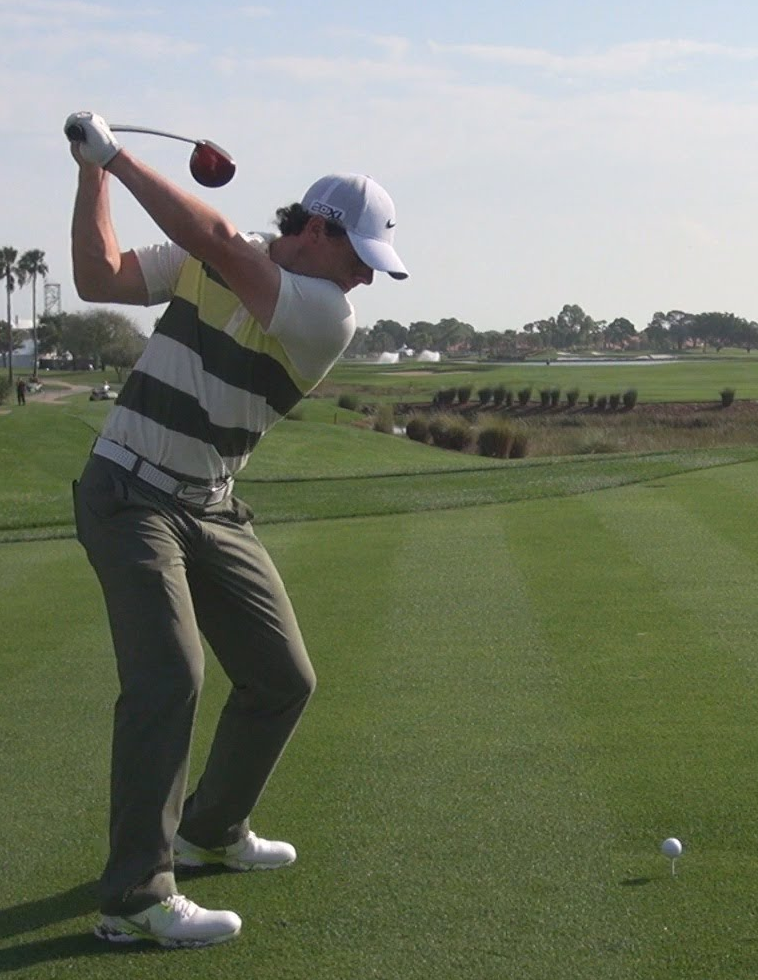
\includegraphics[width=.95\textwidth]{images/swing}
\end{center}
\end{minipage}\hfill
\begin{minipage}[c]{.33\linewidth}
\begin{center}
%\includegraphics[width=.9\textwidth]{images/situation}
\end{center}
\end{minipage}\hfill
\begin{minipage}[c]{.45\linewidth}
\begin{center}
%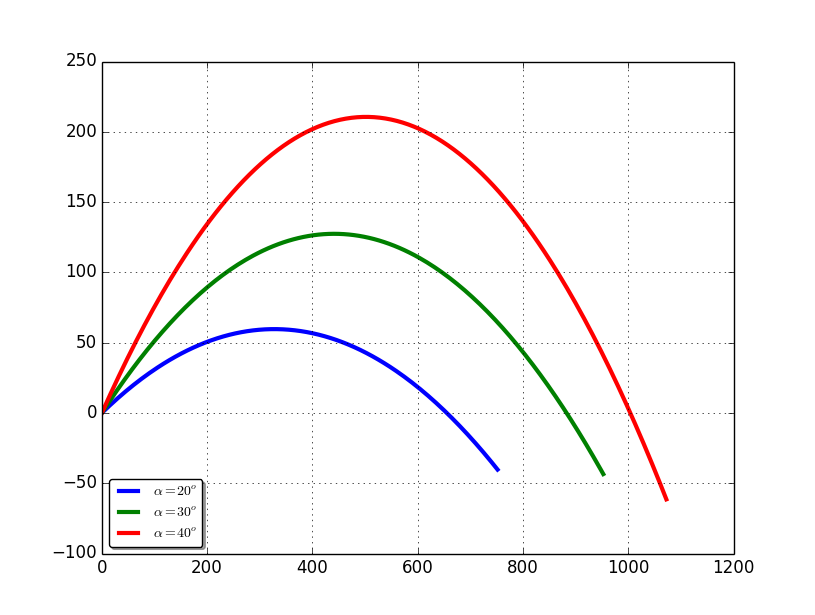
\includegraphics[width=.95\textwidth]{images/tir_alpha}
\end{center}
\end{minipage}
\vspace{.5cm}

On reprend le cas du mouvement d'un swing de golf. On prend maintenant en compte les forces de frottements dus à l'air. 

\begin{savoir}
Problème dynamique à une dimension,  linéaire ou non, conduisant à la résolution approchée d’une équation différentielle ordinaire par la méthode d’Euler.
\end{savoir}



\setlength{\parskip}{0ex plus 0.2ex minus 0ex}
 \renewcommand{\contentsname}{}
 \renewcommand{\baselinestretch}{1}

\tableofcontents

 \renewcommand{\baselinestretch}{1.2}
\setlength{\parskip}{2ex plus 0.5ex minus 0.2ex}





\section{Mise en place du problème}

Une grande part des problèmes scientifiques se modélisent par une équation différentielle dont on cherche la solution pour dimensionner ou comprendre le phénomène.

Quand les équations sont simples (linéaires d'ordre 1 ou 2) la résolution analytique est aisée, mais nombre de modélisations conduisent à des équations non linéaires.  Ce cours a pour objectif de proposer des méthodes pour déterminer une solution approchée.

\subsection{Problème de Cauchy}

Le problème de Cauchy consiste à trouver les fonctions $  {Y}$ de $[0, T] \to \mathbb{R}^N$, telles que :
\[\left\{
\begin{matrix}
\dfrac{\d  {Y}}{\d t} =   {F}(t,  {Y}) \\
  {Y}(t_0)=  {Y_0}
\end{matrix}\right.
\]
où $t_0\in [0, T]$ et $  {Y_0}\in\mathbb{R}^N$ sont des données.

La plupart des systèmes d'équations différentielles de tout ordre peuvent se mettre sous cette forme de système d'équations différentielles du premier ordre\footnote{à l'exception des équations différentielles implicites} (un exemple sera traité plus loin).

\subsection{Existence et unicité de la solution}
\textbf{Théorème de Cauchy-Lipschitz :} soit $  {F}$ une fonction de $[0,T]\times\mathbb{R}^N \to \mathbb{R}^N$ continue et lipschitzienne en $  {Y}$. 

Alors, $\forall~ t_0\in [0, T]$ et $\forall~   {Y_0}\in\mathbb{R}^N$, le problème de Cauchy admet une solution unique définie sur $[0,T]$.


\bigskip
\textbf{Rappel :} $  {F}$ lipschitzienne en $  {Y}$ : 
\[\exists~ k>0\textrm{ tel que,} \forall~   {Y}\in\mathbb{R}^N, \forall~   {Z}\in\mathbb{R}^N, \forall~ t\in[0,T],\qquad \Vert   {F}(t,  {Y})-  {F}(t,  {Z})\Vert \leq k \Vert    {Y}-  {Z} \Vert\]


\subsection{Résolution numérique}
L'objectif est d'obtenir une solution approchée au problème de Cauchy pour une discrétisation temporelle de l'intervalle donné. 
La démarche s'appuie sur la forme initiale de l'équation différentielle où il est facile de voir que la fonction $  {F}(t,  {Y})$ traduit l'évolution de $  {Y}$, c'est-à-dire la pente de la courbe $  {F}(t,  {Y})(t)$. Les schémas d'intégration numériques exploitent $  {F}(t,  {Y})$ pour traduire l'évolution sur un pas de temps.

En notant $h$ le pas de temps et $N$ le nombre de pas de temps, l'intervalle est discrétisé par $t_0=0$, $t_1=h$, ..., $t_N = Nh$.

Sur un sous-intervalle donné, on cherche à déterminer la solution sous la forme :\[\int\limits_{t_i}^{t_{i+1}} \dfrac{\d  {Y}}{\d t} \d t = \int\limits_{t_i}^{t_{i+1}}   {F}(t,  {Y})\d t \qquad\qquad\textrm{on en déduit que :}  {Y}_{i+1} =   {Y}_{i} +  \int\limits_{t_i}^{t_{i+1}}   {F}(t,  {Y})\d t \]

%\parpic[r]{
%\begin{tikzpicture}\node  {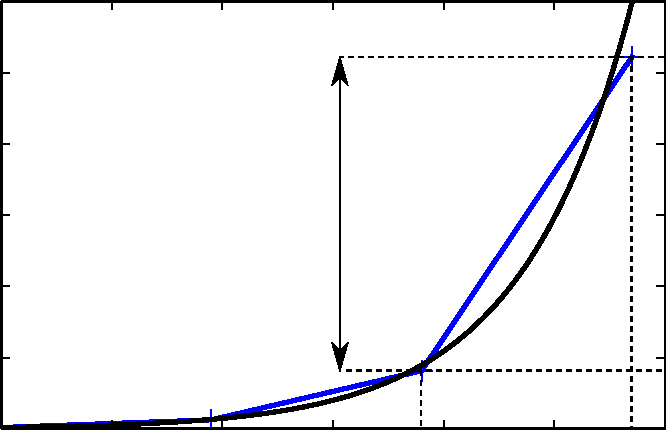
\includegraphics[width=5cm]{illu_tangente1}};
%\node at (.7,-2) {$  {t}_{i}$};
%\node at (2.4,-2) {$  {t}_{i+1}$};
%\node[right] at (2.7,1) {$  {Y}_{i+1}$};
%\node[right] at (2.7,-1.2) {$  {Y}_{i}$};
%\node[left] at (0,0) {$h  {\Phi}( t_j,  {Y}_j,h)$};
%\end{tikzpicture}}


Les méthodes de résolution numérique des équations différentielles sont basées sur des techniques d'estimation de l'intégrale de la fonction $  {F}$.

On s'intéressera dans ce cours aux méthodes de résolution à un pas qui se mettent sous la forme générale :
\[ \displaystyle \left\{\begin{matrix}
  {Y}_{i+1} =   {Y}_{i} +  h  {\Phi}( t_j,  {Y}_j,h)\\
  {Y}(t_0)=  {Y_0}
\end{matrix}\right. \]
où il faudra choisir $  {\Phi}$ intelligemment.

La fonction $  {\Phi}$ représente la pente de la droite permettant de passer de $  {Y}_{i}$ à $  {Y}_{i+1}$.




\section{Méthodes à un pas}
L'exemple élémentaire qui servira de support est la résolution de l'équation différentielle :\\ $\dot y(t) + y(t) = 0$ avec $y(0)=1$, dont la solution exacte est $y(t)=e^{-t}$.

\subsection{Méthode d'Euler explicite}
\subsubsection{Méthode}

%\parpic[r]{
%\begin{tikzpicture}\node  {\includegraphics[width=5cm]{illu_tangente2_}};
%\node at (0,-2) {$  {t}_{i}$};
%\node at (1.3,-2) {$  {t}_{i+1}$};
%\node[right] at (2.7,-.4) {$  {Y}_{i+1}$};
%\node[right] at (2.7,-1.1) {$  {Y}_{i}$};
%\end{tikzpicture}}



La première façon d'approximer l'intégrale est de réaliser une méthode des rectangles à gauche. \\
Ainsi $\int\limits_{t_i}^{t_{i+1}}   {F}(t,  {Y})\d t = h   {F}(t_i,  {Y}_i)$.

On en déduit que $  {\Phi} =   {F}(t_i,  {Y}_i) $

Ainsi la relation de récurrence générale est : \\$  {Y}_{i+1} =   {Y}_{i} + h  {F}(t_i,  {Y}_i)$

La pente permettant de passer de $  {Y}_{i}$ à $  {Y}_{i+1}$ est la valeur de $  {F}(t_i,  {Y}_i)$ comme l'illustre la figure ci-contre où le champ de la fonction $  {F}$ est tracée.

%\picskip{1}
%\bigskip

On peut aussi exprimer la relation sous la forme : $  {F}(t_i,  {Y}_i)=\dfrac{\d  {Y}}{\d t}(t_i) \simeq \dfrac{  {Y}_{i+1}-  {Y}_i}{h}$.  


\subsubsection{Propriétés (voir Annexe mathématique pour les définitions)}
\paragraph{Stabilité} $  {\Phi}$ est lipschitzienne donc le schéma est stable.

\paragraph{Consistance} L'erreur de consistance est $c_i =   {Y}_{ex}(t_{i+1})-  {Y}_{ex}(t_i)-h  {F}( t_i,  {Y}_{ex}(t_i))$

Or le développement de Taylor-Lagrange donne : 
$  {Y}_{ex}(t_{i}+h)=  {Y}_{ex}(t_{i+1}) = 
  {Y}_{ex}(t_{i})+h  {\dot Y}_{ex}(t_{i}) + \dfrac{h^2}{2}   {\ddot Y}_{ex}(\xi)$ avec $\xi\in[t_i,t_i+h]$.

Or $  {\dot Y}_{ex} =   {\Phi}(t_i,  {Y}_{ex}(t_i),h) =   {F}(t_i,  {Y}_{ex}(t_i))$

On en déduit que $c_i = \dfrac{h^2}{2}   {\ddot Y}_{ex}(\xi)$ avec $\xi\in[t_i,t_i+h]$

Ainsi la méthode est consistante. Comme elle est stable, on en déduit qu'elle est convergente. 

L'expression de l'erreur de consistance indique que la méthode est d'ordre 1.

\subsubsection{Application}


  {\'Ecrire la relation de récurrence de la méthode d'Euler sur l'exemple.}


  {Montrer que pour certaines valeurs de $h$, la solution peut présenter des problèmes. Justifier et commenter les courbes de la \ref{euler_expl}.}

\begin{figure}[!ht]
\centering
%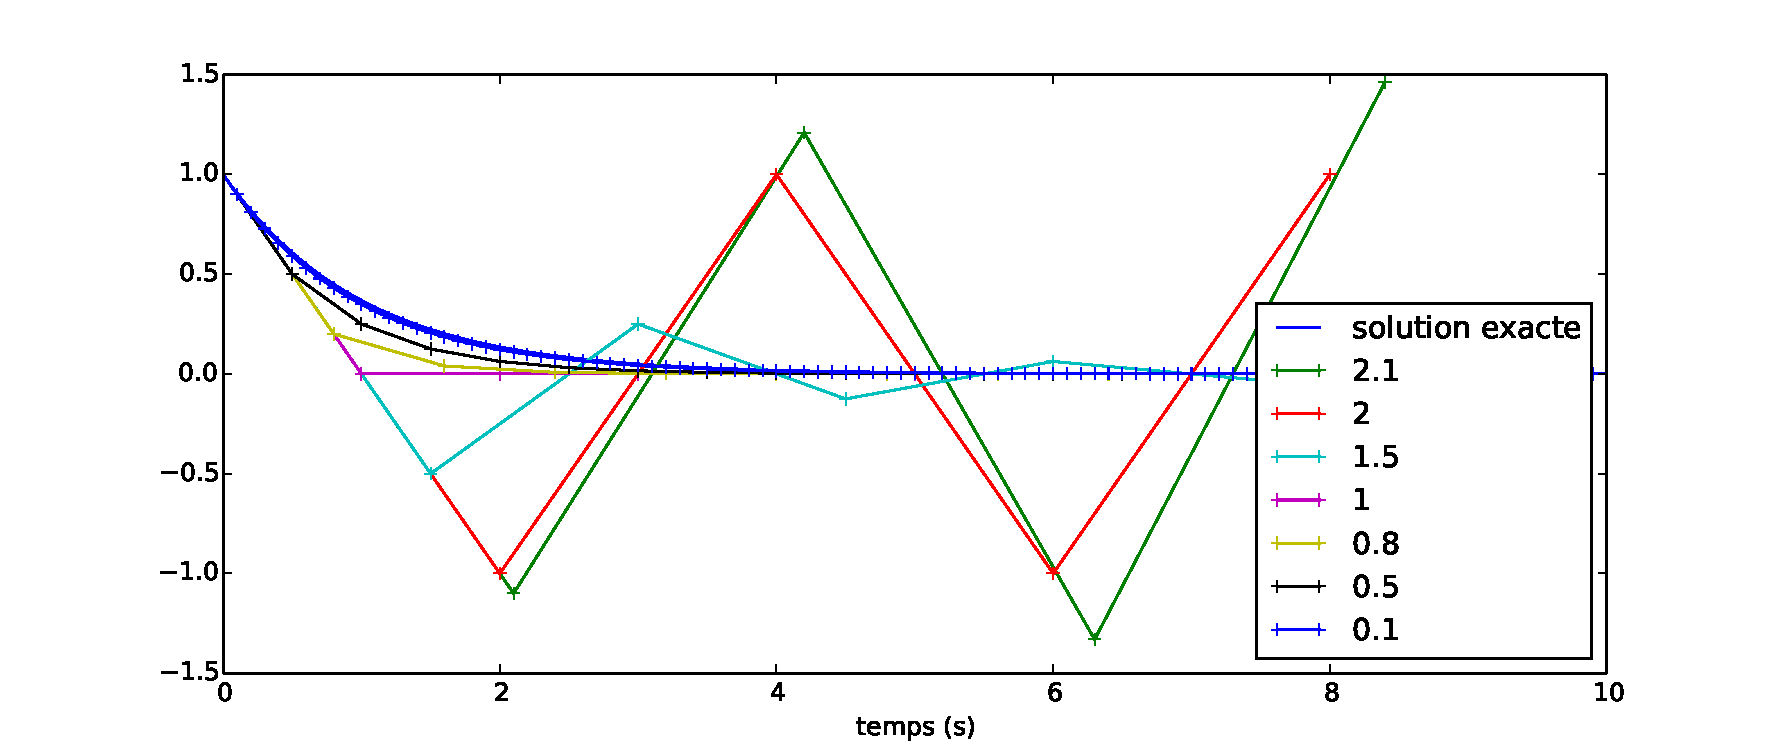
\includegraphics[width=.8\linewidth]{euler_explicite_}

%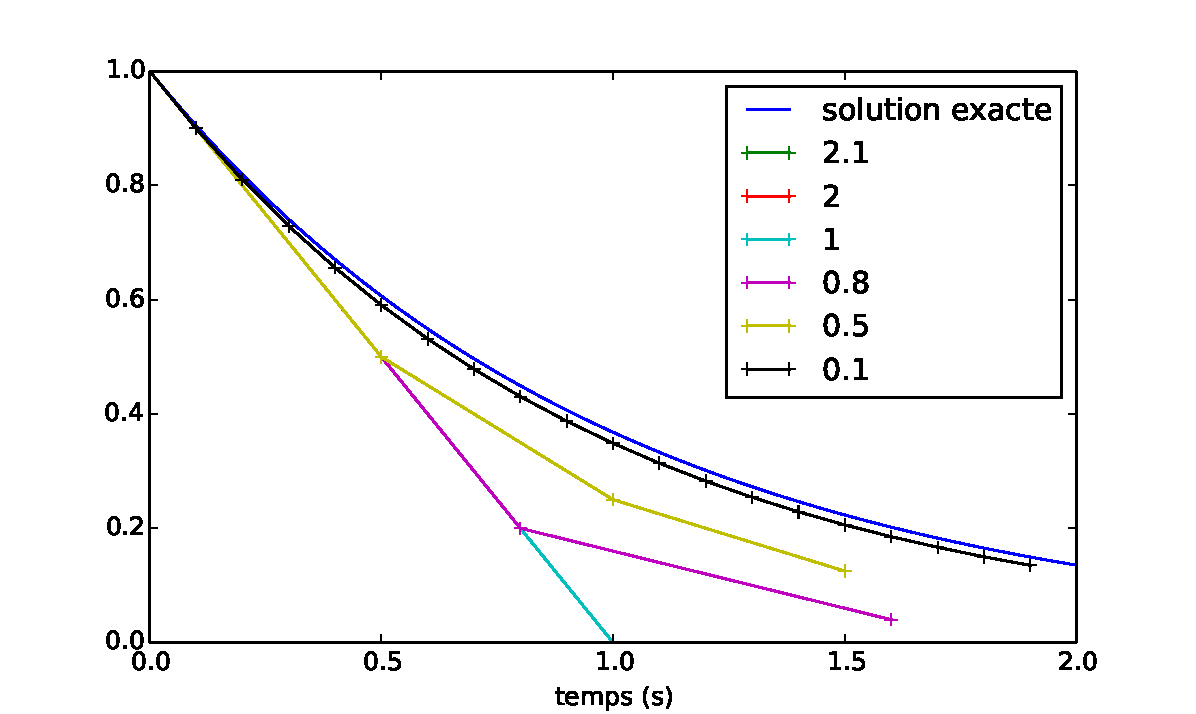
\includegraphics[width=.5\linewidth]{euler_explicite_zoom}
\caption{Solution de l'application pour le schéma Euler explicite.}
\label{euler_expl}
\end{figure}

Le tableau suivant donne l'erreur comme étant le maximum de l'écart entre la solution exacte et la solution approchée ainsi que le temps de calcul pour différentes valeurs du pas de temps.

\begin{center}
\begin{tabular}{*7{|c}|}
\hline
%$h$ &   {e-1} &\num{e-2} &\num{e-3} &\num{e-4} &\num{e-5} &\num{e-6} \\ \hline
%$N$ pas de temps & \num{100} & \num{1000} &\num{10000} &\num{100000} &\num{1000000} &\num{10000000} \\ \hline
%Erreur & \num{4.1e-1}& \num{4.9e-2}& \num{5.0e-3}& \num{5.0e-04}& \num{5.0e-5}& \num{5.0e-06}\\ \hline
%Temps (s) & \num{5.2e-3} & \num{1.6e-2}& \num{7.8e-2}& \num{5.7e-1}& \num{5.0}& \num{50} \\ \hline
\end{tabular}
\end{center}

On constate que l'erreur évolue linéairement en fonction du pas de temps ainsi que le temps de calcul (complexité en $O(N)$ car une seule boucle).

Il faut descendre à un pas de temps très faible avant d'obtenir un niveau d'erreur satisfaisant. On voit bien ici la limitation des méthodes d'ordre 1.


%\bigskip
%\parpic[r]{
%\begin{tikzpicture}\node  {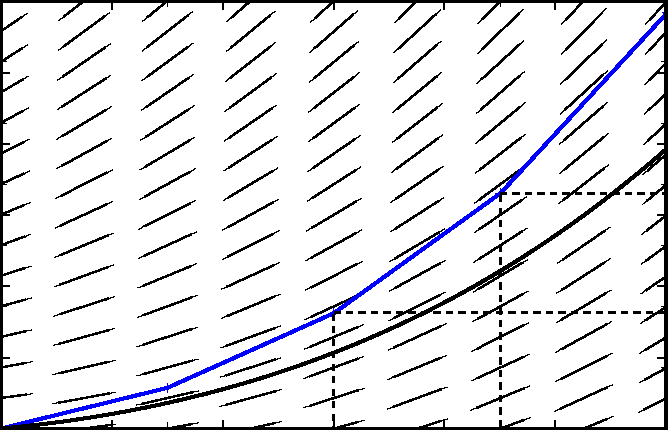
\includegraphics[width=5cm]{illu_tangente3_}};
%\node at (0,-2) {$  {t}_{i}$};
%\node at (1.3,-2) {$  {t}_{i+1}$};
%\node[right] at (2.7,0) {$  {Y}_{i+1}$};
%\node[right] at (2.7,-0.7) {$  {Y}_{i}$};
%\end{tikzpicture}}

\noindent\begin{minipage}{10cm}
\subsection{Méthode d'Euler implicite}
%\vspace{-2ex}
\subsubsection{Méthode}
%\vspace{-3ex}
La seconde façon d'approximer l'intégrale est de réaliser une méthode des rectangles à droite. \\
Ainsi $\int\limits_{t_i}^{t_{i+1}}   {F}(t,  {Y})\d t = h   {F}(t_{i+1},  {Y}_{i+1})$.
\end{minipage}

%\picskip{1}

On en déduit que $  {\Phi} =   {F}(t_{i+1},  {Y}_{i+1}) $

Ainsi la relation de récurrence générale est : $  {Y}_{i+1} =   {Y}_{i} + h  {F}(t_{i+1},  {Y}_{i+1})$

La pente permettant de passer de $  {Y}_{i}$ à $  {Y}_{i+1}$ est la valeur de $  {F}(t_{i+1},  {Y}_{i+1})$ comme l'illustre la figure ci-contre où le champ de la fonction $  {F}$ est tracée.

%\picskip{1}
%\bigskip

On peut aussi exprimer la relation sous la forme : $  {F}(t_{i+1},  {Y}_{i+1})=\dfrac{\d  {Y}}{\d t}(t_{i+1}) \simeq \dfrac{  {Y}_{i+1}-  {Y}_i}{h}$.  



%\medskip
On remarque que le second membre dépend aussi de $  {Y}_{i+1}$. Il faut donc dans les cas non linéaires se ramener à un problème stationnaire à résoudre avec la méthode de Newton sur :
$  {Y}_{i+1} -   {Y}_{i} - h  {F}(t_{i+1},  {Y}_{i+1}) = 0$ ce qui alourdit notablement le calcul. Dans les cas linéaires, il faut au moins une inversion, ce qui est aussi très lourd pour les problèmes de grande dimension. Il faut donc retenir qu'une méthode implicite est généralement plus coûteuse qu'une méthode explicite à pas de temps égal.

\subsubsection{Propriétés}
De même que pour la méthode explicite, la méthode est convergente et d'ordre 1.

\subsubsection{Application}

  {\'Ecrire la relation de récurrence de la méthode d'Euler implicite sur l'exemple.}

  {Montrer que quelle que soit la valeur de $h$, la solution ne peut plus présenter les mêmes problèmes qu'en explicite.}

La solution approchée pour différents pas de temps est donnée sur la \ref{euler_impl}.

\begin{figure}[!ht]
\centering
%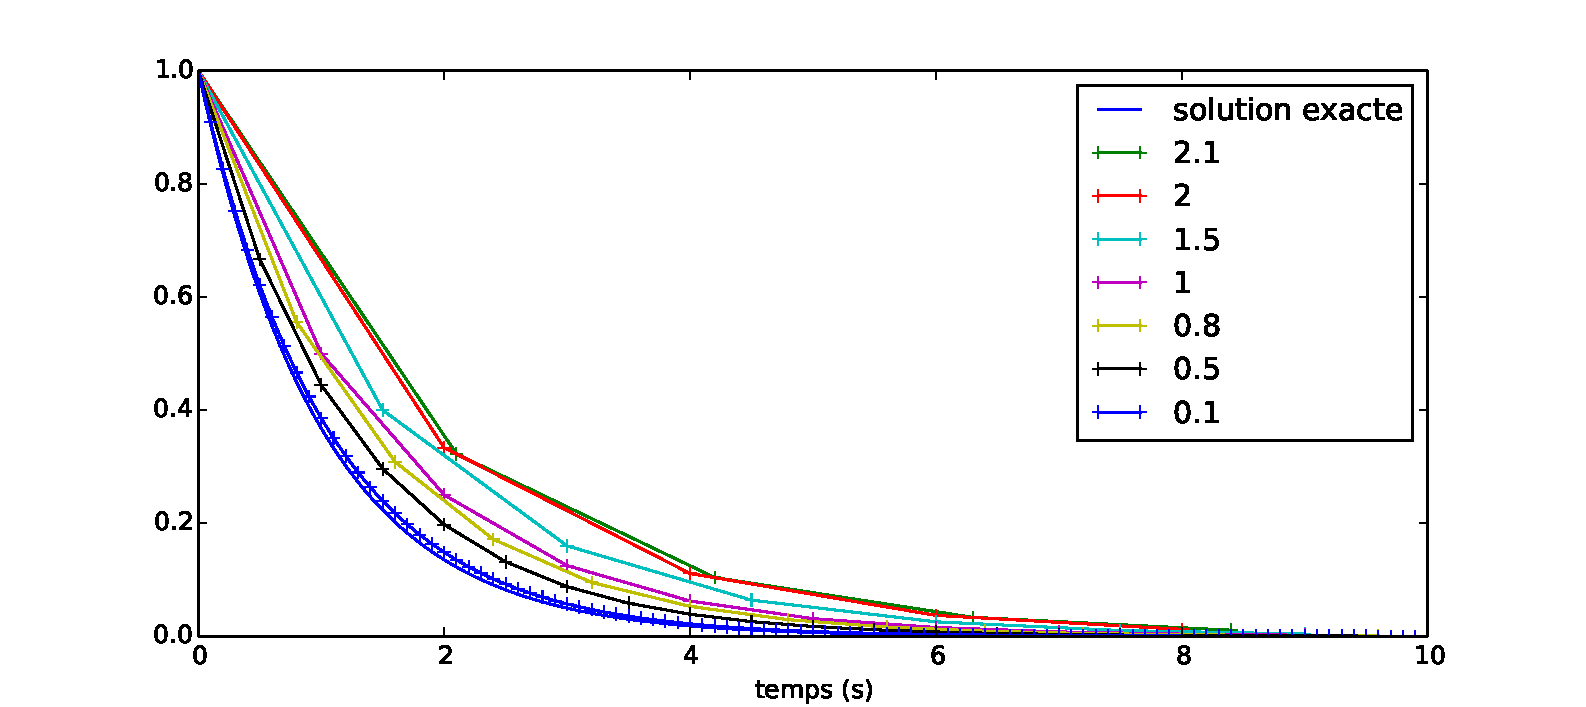
\includegraphics[width=.7\linewidth]{euler_implicite}

\caption{Solution de l'application pour le schéma Euler implicite.}
\label{euler_impl}
\end{figure}

Le tableau suivant donne l'erreur comme étant le maximum de l'écart entre la solution exacte et la solution approchée ainsi que le temps de calcul pour différentes valeurs du pas de temps.

\begin{center}
\scalebox{.9}{\begin{tabular}{*7{|c}|}
\hline
%$h$ & \num{e-1} &\num{e-2} &\num{e-3} &\num{e-4} &\num{e-5} &\num{e-6} \\ \hline
%$N$ pas de temps & \num{100} & \num{1000} &\num{10000} &\num{100000} &\num{1000000} &\num{10000000} \\ \hline
%Erreur & \num{5.9e-1}& \num{5.0e-2}& \num{5.0e-3}& \num{5.0e-04}& \num{5.0e-05}& \num{5.0e-06}\\ \hline

%Temps (s) & \num{5.2e-3} & \num{3.1e-2}& \num{3.7e-1}& \num{3.7}& \num{37}& \num{370} \\ \hline
\end{tabular}}
\end{center}

On constate que l'erreur évolue linéairement en fonction du pas de temps ainsi que le temps de calcul (complexité en $O(N)$ car une seule boucle). Le temps de calcul est cependant plus important à cause de la résolution de l'équation avec l'algorithme de Newton (on aurait pu inverser analytiquement la relation dans ce cas d'école).

Il faut descendre à un pas de temps très faible avant d'obtenir un niveau d'erreur satisfaisant. On voit bien ici la limitation des méthodes d'ordre 1.


\subsection{Méthode de Runge-Kutta}
Les méthodes d'Euler peuvent être vu comme une approximation du développement de Taylor-Lagrange à l'ordre 1. Pour augmenter la précision, une solution pourrait être d'augmenter l'ordre de développement ; c'est cependant impossible sans les expressions des dérivées n-ième de la fonction $  {F}$.

Le schéma de Runge-Kutta permet d'obtenir des méthodes d'ordres plus élevés sans utiliser les fonctions dérivées de $  {F}$.

\subsubsection{Expression générale des méthodes de Runge-Kutta explicites}

La méthode générale consiste à déterminer $  {\Phi}$ à partir d'approximations successives.

On choisit $\displaystyle   {\Phi}(\tau,  {Y},h) = \sum_{i=1}^q a_i k_i(\tau,  {Y},h)$ avec\\
$k_1(\tau,  {Y},h) =   {F}(\tau,  {Y})$\\
pour $i\geq 2,\qquad k_i(\tau,  {Y},h) =   {F}(\tau+\alpha_ih,   {Y}+\sum_{j=1}^{i-1} \beta_{ij} k_j(\tau,  {Y},h))$

On choisit les paramètres $q$, $a_i$, $\alpha_i$ et $\beta_{ij}$ pour que la méthode soit d'ordre $p$.

\medskip
On remarque que la méthode d'Euler explicite est le cas particulier de Runge-Kutta d'ordre 1.

En pratique, on va rarement au delà de l'ordre 4.

\subsubsection{Runge-Kutta d'ordre 2 (RK2) -- Méthode de Heun}
Le relation de récurrence est $  {Y}_{i+1} =   {Y}_{i} + \dfrac{h}{2}  {F}(t_{i},  {Y}_{i})+ \dfrac{h}{2}  {F}(t_{i}+h,  {Y}_{i}+h  {F}(t_{i},  {Y}_{i}))$.\\
On a donc pris $  {\Phi}(\tau,  {Y},h) = \dfrac{1}{2}(k_1+k_2)$ avec :\\
$k_1=   {F}(t_{i},  {Y}_{i})$ et $k_2=  {F}(t_{i}+h,  {Y}_{i}+h k_1)$.

Cette relation est une intégration de type trapèze entre la valeur au pas $i$ et la valeur du pas $i+1$ estimée à partir d'une méthode d'Euler explicite. 

La solution approchée de l'application pour différents pas de temps est donnée sur la \ref{heun}.

\begin{figure}[!ht]
\centering
%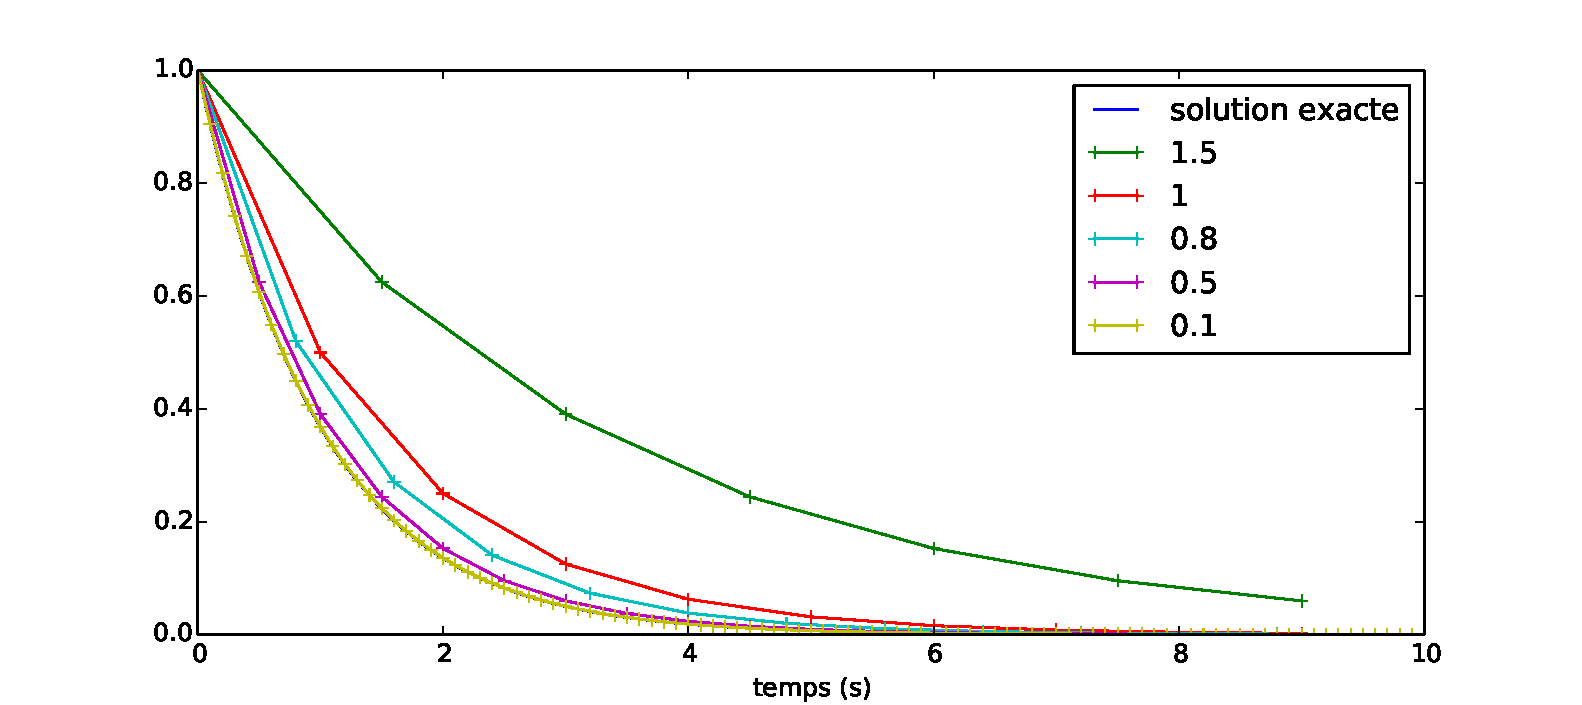
\includegraphics[width=.7\linewidth]{heun}

\caption{Solution de l'application pour le schéma de Heun.}
\label{heun}
\end{figure}

Le tableau suivant donne l'erreur comme étant le maximum de l'écart entre la solution exacte et la solution approchée ainsi que le temps de calcul pour différentes valeurs du pas de temps.

\begin{center}
\scalebox{.9}{
\begin{tabular}{*7{|c}|}
\hline
%$h$ & \num{e-1} &\num{e-2} &\num{e-3} &\num{e-4} &\num{e-5} &\num{e-6} \\ \hline
%$N$ pas de temps & \num{100} & \num{1000} &\num{10000} &\num{100000} &\num{1000000} &\num{10000000} \\ \hline
%Erreur & \num{1.8e-2}& \num{1.7e-4}& \num{1.7e-6}& \num{1.7e-8}& \num{1.7e-10}& \num{1.7e-12}\\ \hline

%Temps (s) & \num{1.5e-3} & \num{1.4e-2}& \num{1.3e-1}& \num{1.2}& \num{12}& \num{120} \\ \hline
\end{tabular}}
\end{center}

On constate que l'erreur évolue quadratiquement en fonction du pas de temps : en divisant le pas de temps par 10, l'erreur diminue d'un facteur 100.

Le temps de calcul est toujours linéaire car la complexité n'a pas augmenté  (complexité en $O(N)$). Il est environ double de la méthode d'Euler explicite puisqu'il y a deux évaluations de $  {F}(t,  {Y})$.


\subsubsection{Runge-Kutta d'ordre 4 (RK4)}

La fonction $  {\Phi}$ est $  {\Phi}(\tau,  {Y},h) = \dfrac{1}{6}(k_1+2k_2+2k_3+k_4)$ avec quatre évaluations successives de $  {F}$ :\\
$k_1(\tau,  {Y},h) =   {F}(\tau,  {Y})$\\
$k_2(\tau,  {Y},h) =   {F}(\tau+\dfrac{h}{2},  {Y}+\dfrac{h}{2}k_1(\tau,  {Y},h))$\\
$k_3(\tau,  {Y},h) =   {F}(\tau+\dfrac{h}{2},  {Y}+\dfrac{h}{2}k_2(\tau,  {Y},h))$\\
$k_4(\tau,  {Y},h) =   {F}(\tau+h,  {Y}+hk_3(\tau,  {Y},h))$\\

La solution approchée pour différents pas de temps est donnée sur la \ref{rk4}.

\begin{figure}[!ht]
\centering
%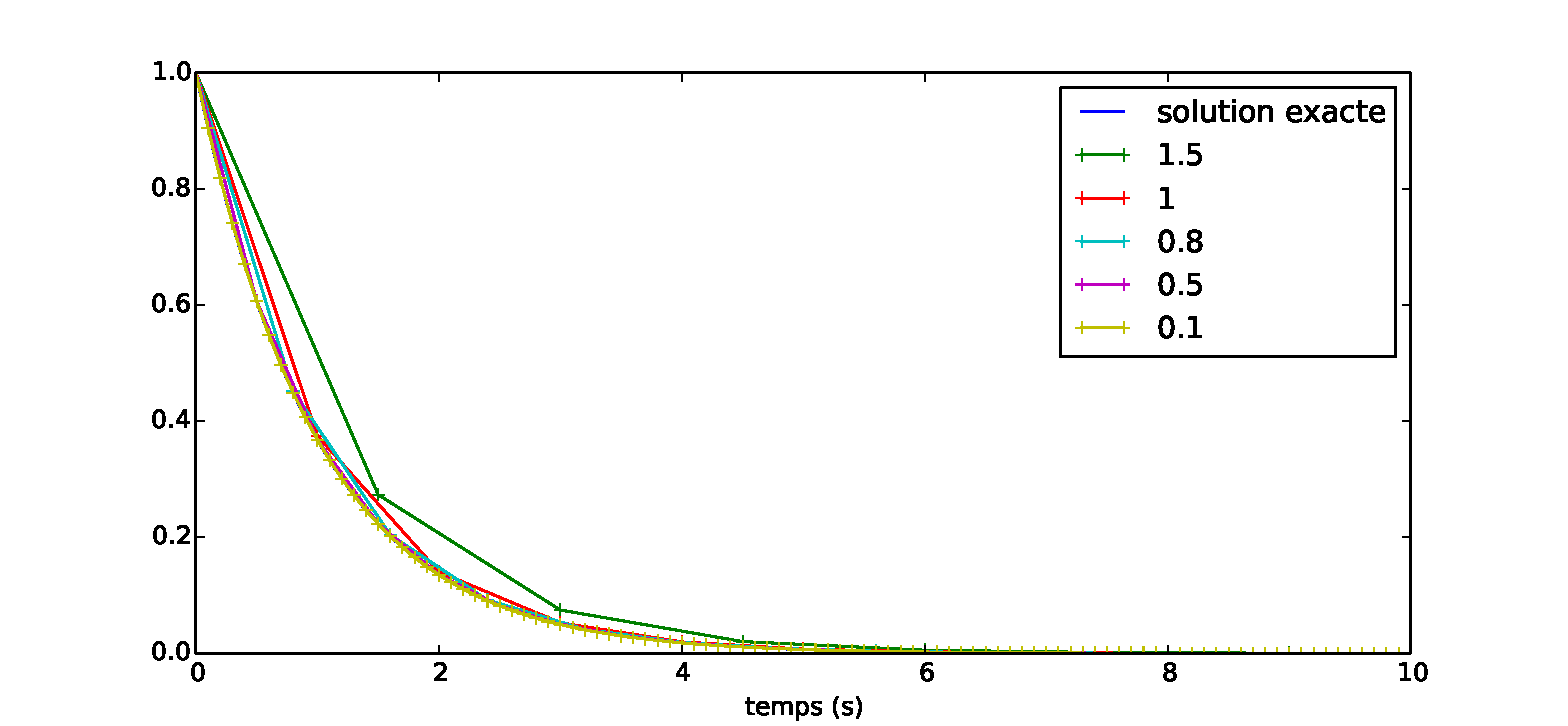
\includegraphics[width=.7\linewidth]{rk4}
\caption{Solution de l'application pour le schéma de Runge-Kutta d'ordre 4.}
\label{rk4}
\end{figure}

Le tableau suivant donne l'erreur comme étant le maximum de l'écart entre la solution exacte et la solution approchée ainsi que le temps de calcul pour différentes valeurs du pas de temps.


\begin{center}
\scalebox{.9}{
\begin{tabular}{*7{|c}|}
\hline
%$h$ & \num{e-1} &\num{e-2} &\num{e-3} \\ \hline
%$N$ pas de temps & \num{100} & \num{1000} &\num{10000} \\ \hline
%Erreur & \num{9.0e-6}& \num{8.4e-10}& \num{9.2e-14}\\ \hline
%Temps (s) & \num{1.7e-3} & \num{1.6e-2}& \num{2.5e-1} \\ \hline
\end{tabular}}
\end{center}

On constate que l'erreur évolue à l'ordre 4 en fonction du pas de temps : en divisant le pas de temps par 10, l'erreur diminue d'un facteur **%\num{10000}.

Le temps de calcul est toujours linéaire car la complexité n'a pas augmentée (complexité en $O(N)$).

\subsection{Conclusion}
En terme de schéma explicite, la méthode de Runge-Kutta à l'ordre 4 est souvent utilisée.

Cependant, vous devez connaître uniquement la méthode d'Euler.

Concernant le choix du pas de temps, il obéit à un compromis entre le temps de calcul, la stabilité et le stockage en mémoire. Le choix de ce pas de temps dépendra essentiellement de la dynamique du système à représenter : si on veut représenter une dynamique à 10 kHz, il faudrait prendre un pas de temps de l'ordre de **%\num{e-5} (10 points par période).
Le choix du pas de temps est souvent fait de manière empirique par expérience de l'ingénieur. 

\section{Mise en forme des systèmes d'équations différentielles}

Nous avons dit au départ que tout système d'équations différentielles pouvait se mettre sous la forme du problème de Cauchy. Traitons quelques exemples.

\subsection{\'Equation harmonique}
Prenons un système masse-ressort. Son équation du mouvement se met sous la forme : \\$\ddot y(t) + \omega_0^2 y(t) = 0$. Les conditions initiales sont $y(0)=1$ et $\dot y(0)=0$.

  {Mettre ce problème sous la forme du problème de Cauchy.}

L'idée est d'introduire des variables supplémentaires. Ici, on introduit la fonction $y_2(t)$ telle qu'elle soit solution de $y_2(t)=\dot{y_1}(t)$ avec $y_1(t)=y(t)$.

L'équation différentielle du système masse-ressort s'écrit ainsi $\dot y_2(t)= - \omega_0^2 y_1(t)$.

En posant $  {Y}(t)=\left(\begin{matrix}
y_1(t)\\y_2(t)
\end{matrix}\right)$, $  {F}(t,  {Y})=\left(\begin{matrix}
y_2(t)\\-\omega_0^2 y_1(t)
\end{matrix}\right)$ et $  {Y}_0=\left(\begin{matrix}
1\\0
\end{matrix}\right)$, on obtient bien la forme du problème de Cauchy. 


La résolution se fait de la même manière que précédemment sauf que cette fois les grandeurs manipulées sont des vecteurs et non plus des scalaires. 

\bigskip
\textbf{Une autre solution classique} permettant de résoudre cette équation différentielle avec la méthode d'Euler explicite est d'appliquer deux fois la définition.

On note $Yp$ la dérivée première. On a $Yp_{i} =\dfrac{Y_{i+1}-Y_i}{h}$

On note $Ypp$ la dérivée seconde. On a $Ypp_{i} =\dfrac{Yp_{i+1}-Yp_i}{h} = \dfrac{Y_{i+2}-2Y_{i+1}+Y_i}{h^2}$.

On en déduit que $Y_{i+2} = (-h^2\omega_0^2 - 1 )Y_i + 2 Y_{i+1}$. On obtient une relation de récurrence directe qui peut être programmée.

Ce schéma est un schéma d'intégration à deux pas qui pourrait s'inscrire dans un cadre plus général des méthodes à plusieurs pas.

\subsection{Système masse-ressort-amortisseur entretenu}
Soit un système masse-ressort-amortisseur soumis à une excitation extérieure harmonique.

L'équation différentielle se met sous la forme générale : $\ddot y(t) + 2\xi\omega_0 \dot y(t)+\omega_0^2 y(t) = f_0\sin(\omega t)$. Les conditions initiales sont $y(0)=1$ et $\dot y(0)=0$ (solution \ref{mrae}).

  {Mettre ce problème sous la forme du problème de Cauchy.}

%\begin{figure}[!ht]
%\centering
%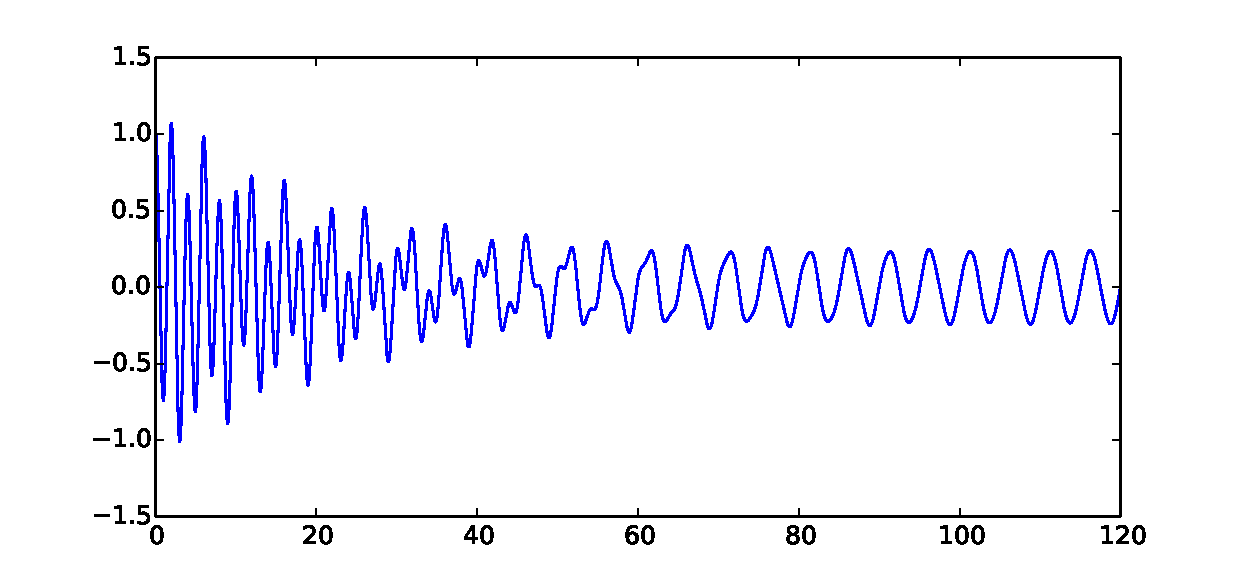
\includegraphics[width=.5\linewidth]{mrae}
%\caption{Solution de l'équation différentielle du système masse-ressort-amortisseur pour $\omega_0=\SI{2}{rad.s^{-1}}$, $\xi=\num{0.015}$, $f_0=\SI{2}{N}$ et $\omega=\SI{5}{rad.s^{-1}}$.}
%\label{mrae}
%\end{figure}

\begin{figure}[!ht]


Solution de l'équation différentielle du système masse-ressort-amortisseur pour ***%$\omega_0=\SI{2}{rad.s^{-1}}$,
% $\xi=\num{0.015}$, $f_0=\SI{2}{N}$ et ***%$\omega=\SI{5}{rad.s^{-1}}$.
% \label{mrae}
%{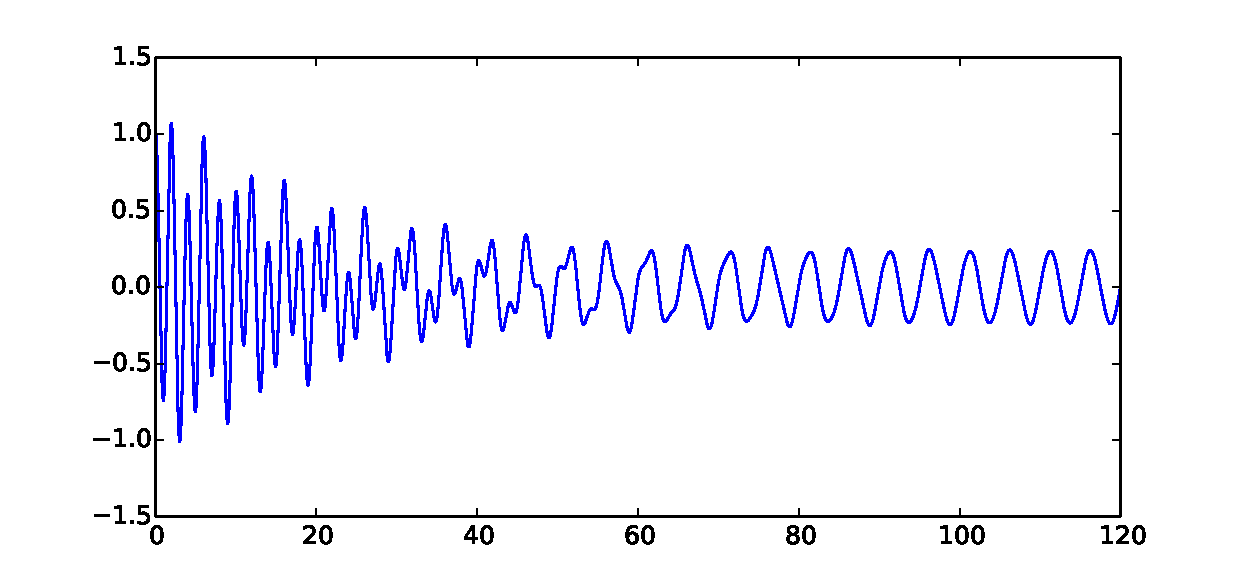
\includegraphics[width=.5\linewidth]{mrae}}
%
%Solution de l'équation différentielle de la réaction de création du glycol.\label{chimie}
%{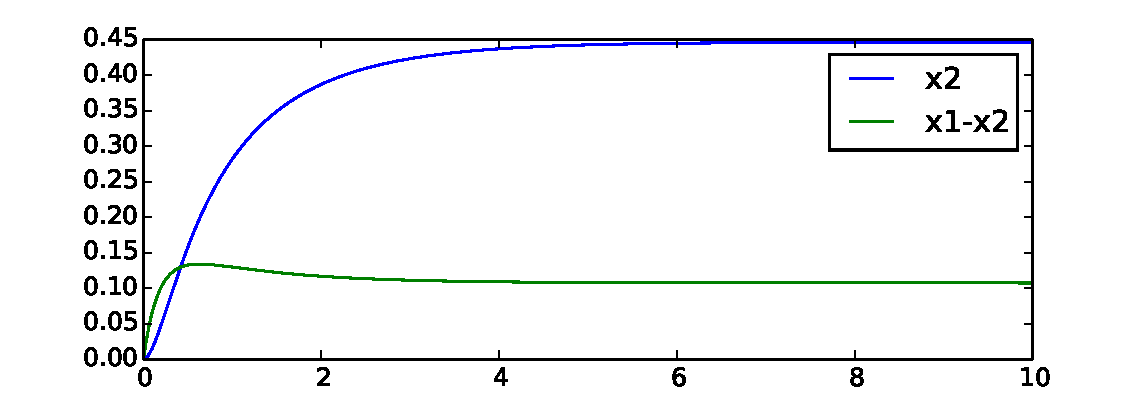
\includegraphics[width=.5\linewidth]{chimie}}
%\caption{Solutions des exemples 2 et 3.}
\end{figure}


\subsection{Création du glycol}
Le glycol (noté $E$) résulte de l'addition d'eau à l'oxyde d'éthylène (noté $O$) en phase gazeuse, selon la réaction
$O + H_2O \xrightarrow{(1)} E$ de constante de vitesse $k_1$. Cette réaction est effectuée à ***%\SI{473}{K}
 sous une pression ***%$P = \SI{15,0}{bar}$
 . Industriellement le temps de passage dans le réacteur ne permet pas d'atteindre l'état d'équilibre thermodynamique
et on constate l'apparition de diéthylèneglycol (noté $D$) produit par la réaction $O+E \xrightarrow{(2)} D$ se déroulant également en phase gazeuse, de constante de vitesse $k_2$. Les réactions sont supposées d'ordre un par rapport à chacun des réactifs et totales. Pour traduire le fait que l'eau réagit moins vite que le glycol $E$ sur l'oxyde d'éthylène $O$, les constantes de vitesse $k_1$ et $k_2$ sont choisies telles que $k_2 = 5k_1$.

Le mélange initial est constitué d'oxyde d'éthylène et d'eau à la concentration molaire ***%$c_0 = \SI{1,00}{mol.L^{-1}}$ 
chacun. On notera $x_1$ l'avancement de la réaction (1) en ***%\si{mol.L^{-1}}
 et $x_2$ l'avancement de la réaction (2) en ***%\si{mol.L^{-1.}}

Les équations différentielles modélisant le mécanisme réactionnel sont (solution \ref{chimie}):
\[ \left\{ \begin{matrix}
\dfrac{\d x_1}{\d t} = k_1 (c_0-x_1-x_2)(c_0-x_1) \\
\dfrac{\d x_2}{\d t} = k_2 (c_0-x_1-x_2)(x_1-x_2) 
\end{matrix}\right.\]

  {Mettre ce problème sous la forme du problème de Cauchy.}


\section{Annexe mathématique}
\subsection{Définitions}
On note $  {Y}_{ex}(t)$ la solution exacte.

\paragraph{Erreur de consistance au pas $i$} \[c_i =   {Y}_{ex}(t_{i+1})-  {Y}_{ex}(t_i)-h  {\Phi}( t_j,  {Y}_{ex}(t_j),h)\]
permet de définir l'erreur réalisée entre l'approximation et la solution exacte au pas de temps $i$.

\paragraph{Méthode consistante} \hfill$\displaystyle\lim_{h\to 0} \sum_{i=1}^N|c_i| = 0$\hfill ~


\paragraph{Méthode stable} Soit le schéma choisi et le schéma perturbé \[ \displaystyle \left\{\begin{matrix}
  {Y}_{i+1} =   {Y}_{i} +  h  {\Phi}( t_j,  {Y}_j,h)\\
  {Y}_{ex}(t_0)=  {Y_0}
\end{matrix}\right. \qquad\qquad
\displaystyle \left\{\begin{matrix}
  {Y}^*_{i+1} =   {Y}^*_{i} +  h  {\Phi}( t_j,  {Y^*}_j,h) + \zeta_i\\
  {Y}_{ex}^*(t_0)=  {Y}^*_0
\end{matrix}\right.
\]

La méthode est stable si :
 \[\displaystyle \exists~ M>0, \qquad 
 \sup\limits_{0 \leq i \leq N} 
 |   {Y}^*_{i}  -   {Y}_{i} 
 | \leq 
 M \left(|  {Y}^*_0-  {Y_0} |+\sum_{i=0}^N |\zeta_i|\right)  \]

\paragraph{Méthode convergente}
\hfill$ \displaystyle\lim_{h\to 0}\left[\sup\limits_{0\leq i\leq N} |  {Y}_{ex}(t_i)-  {Y}_i| \right] = 0$\hfill ~


\paragraph{Ordre de convergence} Une méthode est dite d'ordre $p$ si $\displaystyle\exists~ M>0, \forall~ i, \qquad |c_i| \leq M h^{p+1}$

\subsection{Propriétés} 

\paragraph{Propriété 1} Une méthode est convergente si et seulement si elle est stable et consistante.

\paragraph{Propriété 2} Si $  {\Phi}$ est lipschitzienne en $  {Y}$ alors le schéma numérique est stable.

%\hspace{0.5cm}\begin{minipage}{14cm}

\noindent
\textbf{Démonstration :}\\
Soit le schéma numérique et le schéma perturbé avec $  {\Phi}$ $k-$lipschitzienne. \\
On a : $|  {Y}^*_{i}  -   {Y}_{i}| = |  {Y}^*_{i-1}  -   {Y}_{i-1} + h(  {\Phi}( t_j,  {Y^*}_j,h)-  {\Phi}( t_j,  {Y}_j,h)) + \zeta_{i-1}|$\\
Or $  {\Phi}$ est $k-$lipschitzienne et par inégalité triangulaire, on obtient \\
$ |  {Y}^*_{i}  -   {Y}_{i}|\leq (1+hk) |  {Y}^*_{i-1}  -   {Y}_{i-1}| + |\zeta_{i-1}|$\\
Par récurrence simple, $ |  {Y}^*_{i}  -   {Y}_{i}|\leq (1+hk)^{i} |  {Y}^*_{0}  -   {Y}_{0}| +\sum_{k=0}^{i-1} |\zeta_{k}|$\\
Comme $1+hk>1$, $1\leq (1+hk)^i \leq (1+hk)^N$, ainsi\\
$\forall~ i,\qquad |  {Y}^*_{i}  -   {Y}_{i}| \leq M  \left(|  {Y}^*_0-  {Y_0} |+\sum_{i=0}^N |\zeta_i|\right) $\\
Donc la borne supérieure est également majorée par ce terme, on en déduit que le schéma est stable.



\begin{thebibliography}{2}
\bibitem{1}{Germain Gondor, Problèmes stationnaires à une dimension du type $f(x) = 0$, Lycée Carnot, Dijon. UPSTI.}
\bibitem{2}{Wack et Al., L’informatique pour tous en classes préparatoires aux grandes écoles, Editions Eyrolles.}
\bibitem{3}{Pierre Debout, Dérivation numérique.}
\bibitem{4}{Marc Derumaux, Damion Iceta, Interpolation, intégration et dérivation numérique, Manipulation de fonctions décrites numériquement, UPSTI.}
%\bibitem{1}{Adrien Petri, \textit{Analyse numérique : Intégration numérique}, Notes de cours de TSI 1, Lycée Rouvière, Toulon.}
\end{thebibliography}
\end{document}


